% !TEX program = xelatex
\documentclass[11pt,a4paper]{ctexart}
% Shared preamble for the assignment reports. Use with:
%   \documentclass[11pt,a4paper]{ctexart}  (XeLaTeX)
%   % Shared preamble for the assignment reports. Use with:
%   \documentclass[11pt,a4paper]{ctexart}  (XeLaTeX)
%   % Shared preamble for the assignment reports. Use with:
%   \documentclass[11pt,a4paper]{ctexart}  (XeLaTeX)
%   \input{../common/preamble.tex}
\usepackage[margin=2.3cm]{geometry}
\setmainfont{texgyretermes}[Extension=.otf,UprightFont=*-regular,BoldFont=*-bold,ItalicFont=*-italic,BoldItalicFont=*-bolditalic]
\setsansfont{texgyreheros}[Extension=.otf,UprightFont=*-regular,BoldFont=*-bold,ItalicFont=*-italic,BoldItalicFont=*-bolditalic]
\setmonofont{texgyrecursor}[Extension=.otf,UprightFont=*-regular,BoldFont=*-bold,ItalicFont=*-italic,BoldItalicFont=*-bolditalic]
\usepackage{amsmath,amssymb,mathtools,bm}
\usepackage{graphicx}
\usepackage{booktabs,multirow,makecell,array,tabularx}
\usepackage[table]{xcolor}
\usepackage[most]{tcolorbox}
\usepackage{enumitem}
\usepackage{listings}
\usepackage{subcaption}
\usepackage{siunitx}
\usepackage[hidelinks]{hyperref}
\usepackage[nameinlink,noabbrev]{cleveref}
\usepackage{float}

\setlength{\emergencystretch}{3em}
\linespread{1.15}
\setlist{leftmargin=*,itemsep=2pt,topsep=3pt}
\graphicspath{{figures/}}

\crefname{figure}{图}{图}
\crefname{table}{表}{表}
\crefname{section}{第}{第}
\creflabelformat{section}{#2#1#3 节}
\crefname{equation}{式}{式}
\crefformat{equation}{式~(#2#1#3)}

\lstset{basicstyle=\ttfamily\footnotesize,columns=fullflexible,breaklines=true,frame=single,
  framerule=0.3pt,rulecolor=\color{black!40},backgroundcolor=\color{black!3},
  keywordstyle=\color{blue!60!black}\bfseries,commentstyle=\color{green!40!black},
  numbers=left,numberstyle=\tiny\color{black!50},xleftmargin=1.5em}

% Interview boxes: question, model answer, common wrong answer.
\newtcolorbox{iqbox}[1]{enhanced,breakable,colback=blue!3,colframe=blue!45!black,boxrule=0.5pt,arc=1.5pt,
  left=4pt,right=4pt,top=3pt,bottom=3pt,fonttitle=\bfseries\small,title={面试追问：#1}}
\newtcolorbox{findingbox}[1][]{enhanced,breakable,colback=green!3,colframe=green!40!black,boxrule=0.5pt,arc=1.5pt,
  left=4pt,right=4pt,top=3pt,bottom=3pt,fonttitle=\bfseries\small,title={结论#1}}
\newtcolorbox{caveatbox}{enhanced,breakable,colback=orange!4,colframe=orange!60!black,boxrule=0.5pt,arc=1.5pt,
  left=4pt,right=4pt,top=3pt,bottom=3pt,fonttitle=\bfseries\small,title={不能推出的结论}}

\newcommand{\authorline}{ShaneLiu04\thanks{GitHub: \url{https://github.com/ShaneLiu04}。代码与原始指标：\url{https://gitee.com/liu-xingyan04/mlsys-infra}。本文基于公开课程材料独立完成，与课程团队无隶属关系。}}

\usepackage[margin=2.3cm]{geometry}
\setmainfont{texgyretermes}[Extension=.otf,UprightFont=*-regular,BoldFont=*-bold,ItalicFont=*-italic,BoldItalicFont=*-bolditalic]
\setsansfont{texgyreheros}[Extension=.otf,UprightFont=*-regular,BoldFont=*-bold,ItalicFont=*-italic,BoldItalicFont=*-bolditalic]
\setmonofont{texgyrecursor}[Extension=.otf,UprightFont=*-regular,BoldFont=*-bold,ItalicFont=*-italic,BoldItalicFont=*-bolditalic]
\usepackage{amsmath,amssymb,mathtools,bm}
\usepackage{graphicx}
\usepackage{booktabs,multirow,makecell,array,tabularx}
\usepackage[table]{xcolor}
\usepackage[most]{tcolorbox}
\usepackage{enumitem}
\usepackage{listings}
\usepackage{subcaption}
\usepackage{siunitx}
\usepackage[hidelinks]{hyperref}
\usepackage[nameinlink,noabbrev]{cleveref}
\usepackage{float}

\setlength{\emergencystretch}{3em}
\linespread{1.15}
\setlist{leftmargin=*,itemsep=2pt,topsep=3pt}
\graphicspath{{figures/}}

\crefname{figure}{图}{图}
\crefname{table}{表}{表}
\crefname{section}{第}{第}
\creflabelformat{section}{#2#1#3 节}
\crefname{equation}{式}{式}
\crefformat{equation}{式~(#2#1#3)}

\lstset{basicstyle=\ttfamily\footnotesize,columns=fullflexible,breaklines=true,frame=single,
  framerule=0.3pt,rulecolor=\color{black!40},backgroundcolor=\color{black!3},
  keywordstyle=\color{blue!60!black}\bfseries,commentstyle=\color{green!40!black},
  numbers=left,numberstyle=\tiny\color{black!50},xleftmargin=1.5em}

% Interview boxes: question, model answer, common wrong answer.
\newtcolorbox{iqbox}[1]{enhanced,breakable,colback=blue!3,colframe=blue!45!black,boxrule=0.5pt,arc=1.5pt,
  left=4pt,right=4pt,top=3pt,bottom=3pt,fonttitle=\bfseries\small,title={面试追问：#1}}
\newtcolorbox{findingbox}[1][]{enhanced,breakable,colback=green!3,colframe=green!40!black,boxrule=0.5pt,arc=1.5pt,
  left=4pt,right=4pt,top=3pt,bottom=3pt,fonttitle=\bfseries\small,title={结论#1}}
\newtcolorbox{caveatbox}{enhanced,breakable,colback=orange!4,colframe=orange!60!black,boxrule=0.5pt,arc=1.5pt,
  left=4pt,right=4pt,top=3pt,bottom=3pt,fonttitle=\bfseries\small,title={不能推出的结论}}

\newcommand{\authorline}{ShaneLiu04\thanks{GitHub: \url{https://github.com/ShaneLiu04}。代码与原始指标：\url{https://gitee.com/liu-xingyan04/mlsys-infra}。本文基于公开课程材料独立完成，与课程团队无隶属关系。}}

\usepackage[margin=2.3cm]{geometry}
\setmainfont{texgyretermes}[Extension=.otf,UprightFont=*-regular,BoldFont=*-bold,ItalicFont=*-italic,BoldItalicFont=*-bolditalic]
\setsansfont{texgyreheros}[Extension=.otf,UprightFont=*-regular,BoldFont=*-bold,ItalicFont=*-italic,BoldItalicFont=*-bolditalic]
\setmonofont{texgyrecursor}[Extension=.otf,UprightFont=*-regular,BoldFont=*-bold,ItalicFont=*-italic,BoldItalicFont=*-bolditalic]
\usepackage{amsmath,amssymb,mathtools,bm}
\usepackage{graphicx}
\usepackage{booktabs,multirow,makecell,array,tabularx}
\usepackage[table]{xcolor}
\usepackage[most]{tcolorbox}
\usepackage{enumitem}
\usepackage{listings}
\usepackage{subcaption}
\usepackage{siunitx}
\usepackage[hidelinks]{hyperref}
\usepackage[nameinlink,noabbrev]{cleveref}
\usepackage{float}

\setlength{\emergencystretch}{3em}
\linespread{1.15}
\setlist{leftmargin=*,itemsep=2pt,topsep=3pt}
\graphicspath{{figures/}}

\crefname{figure}{图}{图}
\crefname{table}{表}{表}
\crefname{section}{第}{第}
\creflabelformat{section}{#2#1#3 节}
\crefname{equation}{式}{式}
\crefformat{equation}{式~(#2#1#3)}

\lstset{basicstyle=\ttfamily\footnotesize,columns=fullflexible,breaklines=true,frame=single,
  framerule=0.3pt,rulecolor=\color{black!40},backgroundcolor=\color{black!3},
  keywordstyle=\color{blue!60!black}\bfseries,commentstyle=\color{green!40!black},
  numbers=left,numberstyle=\tiny\color{black!50},xleftmargin=1.5em}

% Interview boxes: question, model answer, common wrong answer.
\newtcolorbox{iqbox}[1]{enhanced,breakable,colback=blue!3,colframe=blue!45!black,boxrule=0.5pt,arc=1.5pt,
  left=4pt,right=4pt,top=3pt,bottom=3pt,fonttitle=\bfseries\small,title={面试追问：#1}}
\newtcolorbox{findingbox}[1][]{enhanced,breakable,colback=green!3,colframe=green!40!black,boxrule=0.5pt,arc=1.5pt,
  left=4pt,right=4pt,top=3pt,bottom=3pt,fonttitle=\bfseries\small,title={结论#1}}
\newtcolorbox{caveatbox}{enhanced,breakable,colback=orange!4,colframe=orange!60!black,boxrule=0.5pt,arc=1.5pt,
  left=4pt,right=4pt,top=3pt,bottom=3pt,fonttitle=\bfseries\small,title={不能推出的结论}}

\newcommand{\authorline}{ShaneLiu04\thanks{GitHub: \url{https://github.com/ShaneLiu04}。代码与原始指标：\url{https://gitee.com/liu-xingyan04/mlsys-infra}。本文基于公开课程材料独立完成，与课程团队无隶属关系。}}

\graphicspath{{../../solutions/cs149/asst2-task-scheduler/artifacts/figures/}}

\title{CS149 Assignment 2 实验报告：\\多核 CPU 上的任务系统与任务图调度（C++17 实现）}
\author{\authorline}
\date{2026 年 10 月}

\begin{document}
\maketitle

\begin{abstract}
Stanford CS149（Fall 2024）Assignment 2 ``Scheduling Task Graphs on a Multi-Core CPU'' 要求实现一个任务执行库，并回答几个看似简单的问题：
线程池比每次新建线程省多少？空闲线程应该自旋还是睡眠？让多个任务批次按依赖关系异步执行，能快多少？
本文用 C++17 在官方 \texttt{IRunnable}/\texttt{ITaskSystem} API 下实现了串行、每次建线程（spawn）、自旋线程池和睡眠线程池（Part~A），
以及支持 \texttt{runAsyncWithDeps}/\texttt{sync} 的依赖图调度器（Part~B，睡眠与自旋两版）。
我按官方结构重写了全部 20 个测试并逐一校验结果，在服务器 12 个独占物理核上独立重复了 3 轮。

主要发现如下。常驻线程池把每次 launch 的固定开销从 spawn 的约 200~µs 降到 1--13~µs，其中自旋池唤醒最快（单任务 0.783~µs，睡眠池 10.8~µs）。
但任务一多，12 个线程会争抢同一个 CAS 状态，自旋池每个空任务要 494~ns，反而是睡眠池（70~ns）的 7 倍。
自旋池空闲时烧满全部 12 个核，睡眠池为 0；在 \texttt{spin\_\allowbreak{}between\_\allowbreak{}run\_\allowbreak{}calls} 上两者墙钟相同（6.28 对 6.37~ms），CPU 时间却差 8 倍。
2 倍超额订阅时，带锁的自旋调度器因为锁持有者被抢占而慢了 766 倍，无锁的自旋池和睡眠池基本不受影响。
12 个 worker 绑满 12 个核时，自旋等待的调用者线程要和一个 worker 分时，造成 32.0~ms 的时间片``平台''；改用 11 个 worker 后降到 18.7~ms。
异步依赖图让独立的 launch 填满彼此的尾部（13 任务/12 线程时快 1.64 倍，理想值 1.83），树形归约达到 work 下界的 96\%。
最后，同一个 64~B 缓存行内的原子计数器在 12 线程时比各占一行慢 19 倍；单个原子分发计数器约 15~ns/次且不随线程数扩展，按 64 个一块分发即可恢复 7.3 倍扩展。
每节附有面试问法与常见错答。仓库原有的 Python 版本作为对照保留。
\end{abstract}

\tableofcontents
\newpage

%====================================================================
\section{背景与作业要求}
\label{sec:intro}

OpenMP、TBB 这类并行运行时都要解决同一个问题：
把一批小任务分给一组线程，让它们尽快做完，同时别让等待本身变成瓶颈。
Stanford CS149（Fall 2024）Assignment 2 ``Scheduling Task Graphs on a Multi-Core CPU''~\cite{cs149} 让学生亲手实现这样一个任务执行库（task system）。

应用程序把工作描述成 \emph{bulk task launch}，即一次批量提交：一个实现了 \texttt{IRunnable::\allowbreak{}runTask(int taskID, int num\_\allowbreak{}total\_\allowbreak{}tasks)} 的对象，加上任务数 $n$。
库负责把这 $n$ 个任务分给工作线程执行。Part~A 只有同步接口 \texttt{run()}；Part~B 增加了
\texttt{runAsyncWithDeps(runnable, n, deps)} 与 \texttt{sync()}，让多个 bulk launch 构成一张有向无环图（DAG），由库按依赖关系调度。

仓库原来的实现是 Python \texttt{threading} 版（\texttt{code/tasksys/systems.py}，15 个测试函数、65 个参数化用例）。
它的结论被 CPython 的 GIL（全局解释器锁，同一时刻只允许一个线程执行 Python 字节码）主导：纯自旋池每次 launch 要 31--50~ms，纯 Python 任务用 8 线程只有 0.92 倍。
这样的数字回答不了作业真正关心的问题，比如``自旋和睡眠哪个快''、``线程池比每次建线程省多少''。
所以本文保留了 Python 版及其测试，另外新增一套与官方 API 一致的 C++17 实现，在服务器 12 个独占物理核上用真实数字回答这些问题，并补充了 9 组扩展实验。
表~\ref{tab:map} 给出官方要求与本文实现的对应关系。

\begin{table}[H]
\centering
\caption{官方作业要求与本文实现（\texttt{cpp/tasksys/}）}
\label{tab:map}
\small
\begin{tabularx}{\linewidth}{>{\raggedright}p{4.5cm}>{\raggedright}X>{\raggedright\arraybackslash}X}
\toprule
官方要求 & 官方要回答的问题 & 本文实现 \\
\midrule
Part A \texttt{TaskSystemSerial} & 基线 & \texttt{TaskSystemSerial} \\
Part A \texttt{TaskSystem\-ParallelSpawn} & 每次 \texttt{run} 建线程的代价；静态还是动态分配任务 & 每次 \texttt{run} 建 $\min(P,n)$ 个线程，原子计数器动态取任务 \\
Part A \texttt{ThreadPoolSpinning} & 常驻线程池能省多少；自旋等待的代价 & 常驻 $P$ 个 worker 自旋；任务由一个打包了 (generation, next) 的 64 位原子变量 CAS 分发 \\
Part A \texttt{ThreadPoolSleeping} & 条件变量让空闲线程睡眠，何时比自旋好 & 同一分发逻辑，worker 在 \texttt{condition\_\allowbreak{}variable} 上睡眠，调用者等待 done 条件变量 \\
Part B \texttt{runAsyncWithDeps}/\texttt{sync} & 依赖跟踪、ready 队列、多个 launch 交错执行 & \texttt{TaskSystemAsync<Spin>}：一把锁保护 launch 表与 ready 队列；sleeping 与 spinning 两个版本 \\
官方测试（\texttt{tests.h}） & 正确性与各系统的性能对比 & 20 个测试全部重写并带结果校验（\cref{sec:tests}） \\
扩展实验 & —— & launch 开销、CPU 代价、超额订阅、粒度、DAG 形状、false sharing、分发计数器、SMT、调用者占核 \\
\bottomrule
\end{tabularx}
\end{table}

%====================================================================
\section{实验环境}
\label{sec:setup}

任务系统的开销多在微秒甚至纳秒级，很容易被机器上的其他负载淹没。所以先交代清楚实验跑在什么样的机器上、用了哪些核、怎么计时。

\begin{table}[H]
\centering
\caption{实验平台}
\label{tab:platform}
\small
\begin{tabularx}{\linewidth}{lX}
\toprule
CPU & 2 $\times$ Intel Xeon Gold 6459C（Sapphire Rapids），每路 32 核，SMT 2；容器可见 128 个逻辑 CPU \\
可用 CPU & cgroup \texttt{cpu.max} = \texttt{1600000 100000}（16 个 CPU 的配额，与其他 6 个实验代理共享）；
本文固定使用 socket~0 的 12 个空闲物理核 \{0,1,2,3,4,6,10,11,14,16,19,23\}，SMT 实验加上兄弟核 $c{+}64$ \\
编译 & g++ 11.4，\texttt{-O3 -march=native -std=c++17 -pthread -Wall}；本机 MinGW-w64 g++ 13（加 \texttt{-static}）用于正确性测试 \\
计时 & \texttt{std::chrono::steady\_\allowbreak{}clock} 墙钟；进程 CPU 时间用 \texttt{getrusage(RUSAGE\_\allowbreak{}SELF)}（Windows 用 \texttt{GetProcessTimes}） \\
绑核 & 整个进程用 \texttt{taskset} 限制在 12 个核上；worker $t$ 用 \texttt{pthread\_\allowbreak{}setaffinity\_\allowbreak{}np} 绑到 \texttt{cores[t mod 12]}；调用者线程不绑核 \\
重复 & 每个测量在进程内重复 3 次；整套实验独立运行 3 轮（\texttt{server12c}、\texttt{\_\allowbreak{}r2}、\texttt{\_\allowbreak{}r3}），文中数字为 9 次的中位数，图中误差棒为最小--最大值 \\
\bottomrule
\end{tabularx}
\end{table}

服务器是共享宿主机，干扰主要有两个来源。第一，其他代理在跑 GPU 实验，它们的 Python 进程不绑核，任何时刻都可能落到本文的核上（实验中 \texttt{top} 看到过一个 100\% 的 Python 进程）。
第二，整个容器共享 16 个 CPU 的配额。cgroup 的 \texttt{nr\_\allowbreak{}throttled} 在第 1 轮中途（超额订阅实验时）为 21，
第 1 轮及随后的 SMT/调用者实验结束时为 31（\texttt{server12c/cgroup\_\allowbreak{}cpu\_\allowbreak{}stat\_\allowbreak{}after.txt}），
说明这段时间里整个容器有 10 个 100~ms 周期用满了配额而被暂停；
第 2、3 轮期间没有再增加（\texttt{server12c\_\allowbreak{}r3/cgroup\_\allowbreak{}cpu\_\allowbreak{}stat\_\allowbreak{}after.txt} 仍为 31）。
第~\ref{sec:caveat}~节会讨论这两类噪声。它们对自旋类实现的影响远大于睡眠类实现，这一点本身也是一个结论。

%====================================================================
\section{方法与实现}
\label{sec:method}

这一节先讲五个任务系统各自怎么实现，重点是常驻线程池里一个很容易写错的竞态；然后介绍 Part~B 的依赖调度，以及测试和扩展实验的设计。

\subsection{API 与五个任务系统}

接口与官方 \texttt{itasksys.h} 一致。Part~A 的系统沿用官方 starter 的做法，把 \texttt{runAsyncWithDeps} 实现为同步 \texttt{run} 加一个递增的 ID，
\texttt{sync()} 为空。所有系统都放在一个头文件 \texttt{cpp/\allowbreak{}tasksys/\allowbreak{}tasksys.h} 里，约 330 行。

\paragraph{Spawn。} 每次 \texttt{run} 创建 $\min(P,n)$ 个 \texttt{std::thread}，每个线程循环执行 \texttt{i = next.fetch\_\allowbreak{}add(1)}，直到 $i\ge n$，最后 \texttt{join}。
动态分配让不均匀的任务自动均衡；代价是每次 launch 都要付创建和销毁线程的系统调用。

\paragraph{线程池的分发状态。} 常驻线程池的难点在于 \emph{launch 之间的竞态}。设想一个 worker 读到了上一个 launch 的计数器，随后被抢占；
等它醒来，调用者已经发布了下一个 launch，它的 \texttt{fetch\_\allowbreak{}add} 就会偷走新 launch 的一个下标，却用旧的 runnable 去执行。
本文的做法是把 generation（第几次 launch）和下一个任务下标打包进同一个 64 位原子变量，用 CAS（比较并交换）认领任务：只有 generation 仍然相同、下标仍小于 $n$ 时，CAS 才会成功。

\begin{lstlisting}[language=C++,caption={分发状态：generation 与下标打包，CAS 认领（tasksys.h）}]
// state_ = (generation << 32) | next_index
bool drain(unsigned g) {               // run tasks of launch g until none left
    bool last = false;
    unsigned long long v = state_.load(std::memory_order_acquire);
    while (gen_of(v) == g) {
        int total = total_.load(std::memory_order_relaxed);
        int i = idx_of(v);
        if (i >= total) break;
        if (!state_.compare_exchange_weak(v, v + 1, std::memory_order_acq_rel)) continue;
        runnable_.load(std::memory_order_relaxed)->runTask(i, total);
        if (done_.fetch_add(1, std::memory_order_acq_rel) + 1 == total) last = true;
        v = state_.load(std::memory_order_acquire);
    }
    return last;
}
\end{lstlisting}

为什么这样就正确了？因为调用者只有在 \texttt{done == total} 之后才会发布下一个 generation，而一个认领成功的任务在完成之前不会让 \texttt{done} 到达 \texttt{total}。
所以 CAS 成功后读到的 runnable，一定属于同一个 launch。

\paragraph{Spinning。} worker 在 \texttt{while(!stop)} 里反复读 \texttt{state\_\allowbreak{}}，有任务就 \texttt{drain}，没有就执行 \texttt{pause}（降低自旋对 SMT 兄弟线程和功耗的影响~\cite{intel}）。
调用者发布 launch 后，自旋等待 \texttt{done == n}。
与官方参考实现一样，根据 Amdahl 定律~\cite{amdahl}，调用者的串行部分（例如 \texttt{spin\_\allowbreak{}between\_\allowbreak{}run\_\allowbreak{}calls} 中的 fib(27)）决定了这类测试的下限。

\paragraph{Sleeping。} worker 在条件变量上等待``generation 变化或 stop''，醒来后 \texttt{drain}。完成最后一个任务的 worker 在锁内写 \texttt{finished\_\allowbreak{}gen}，然后 \texttt{notify\_\allowbreak{}one}；
调用者在另一个条件变量上等待。所有共享谓词都在同一把锁内修改，这样不会丢失唤醒（lost wakeup）；所有 wait 都带谓词，防止虚假唤醒。

\subsection{Part B：带依赖的异步 launch}

Part~B 要让多个 launch 按依赖关系交错执行。下面是 worker 主循环的核心部分：

\begin{lstlisting}[language=C++,caption={Part B worker 主循环（sleeping 版，tasksys.h 节选）}]
lk.lock();
work_cv_.wait(lk, [&] { return stop_ || !ready_.empty(); });
auto [id, L] = ready_.front();
int i = L->next++;                         // take one task of the front ready launch
if (L->next == L->total) ready_.pop_front();
lk.unlock();
L->r->runTask(i, L->total);
lk.lock();
if (++L->done == L->total) finish(id, L);  // decrement dependents' pending; push newly ready
lk.unlock();
\end{lstlisting}

每个 launch 记录两样东西：\texttt{pending}（尚未完成的依赖数）和 \texttt{dependents}（依赖它的 launch）。
提交时，已经完成的依赖直接忽略（它们已从 \texttt{live\_\allowbreak{}} 表中删除），否则把自己挂到依赖的 \texttt{dependents} 上；\texttt{pending == 0} 的 launch 进入 ready 队列。
worker 每次从队首 launch 取 \emph{一个} 任务。队首 launch 的任务被取完后，下一个 ready launch 的任务立刻接上，
这就是独立 launch 能``互相填满尾部空闲''的机制。
\texttt{finish} 在锁内递减后继的 \texttt{pending}，减到 0 的入队并 \texttt{notify\_\allowbreak{}all}；未完成的 launch 数降为 0 时唤醒 \texttt{sync}。
spinning 版用同一套数据结构，只是把两处条件变量换成对原子计数器 \texttt{ready\_\allowbreak{}count\_\allowbreak{}}/\texttt{unfinished\_\allowbreak{}} 的轮询。
Part~B 的同步 \texttt{run} 就是 \texttt{runAsyncWithDeps(r, n, \{\}) + sync()}。

\subsection{官方测试负载}
\label{sec:tests}

官方 starter 的 \texttt{tests.h} 不在仓库中，所以本文按其结构重写了 20 个测试（\texttt{cpp/\allowbreak{}tasksys/\allowbreak{}tests.h}），参数见表~\ref{tab:tests}。
调度器写错时往往不会崩溃，只会悄悄算错，所以每个测试都校验结果：ping-pong 与归约树用 32 位 LCG 迭代（整数运算，结果确定），抽样元素与串行重算比较；
fibonacci 比较每个任务的返回值；Mandelbrot 抽样像素与串行重算比较；math ops 用相同的浮点表达式逐位比较。任何一处不一致都会让进程以非零码退出。

\begin{table}[H]
\centering
\caption{重写的官方测试（scale = 1 时的参数）}
\label{tab:tests}
\small
\begin{tabularx}{\linewidth}{>{\raggedright}p{5.2cm}X}
\toprule
测试 & 结构 \\
\midrule
\texttt{super\_\allowbreak{}super\_\allowbreak{}light(\_\allowbreak{}async)} & 400 次 launch × 64 任务，32K 元素拷贝（0 次迭代），相邻 launch 有依赖（ping-pong） \\
\texttt{super\_\allowbreak{}light(\_\allowbreak{}async)} & 同上，每元素 1 次 LCG \\
\texttt{ping\_\allowbreak{}pong\_\allowbreak{}equal(\_\allowbreak{}async)} & 64 次 launch × 64 任务，128K 元素，每元素 32 次 LCG \\
\texttt{ping\_\allowbreak{}pong\_\allowbreak{}unequal(\_\allowbreak{}async)} & 同上，任务 $i$ 的迭代数 $\approx 2\cdot 32\,(i+1)/n$（线性递增的不均衡） \\
\texttt{recursive\_\allowbreak{}fibonacci(\_\allowbreak{}async)} & 8 次 launch × 256 任务，每任务递归 fib(23)；async 版各 launch 独立 \\
\texttt{math\_\allowbreak{}operations\_\allowbreak{}in\_\allowbreak{}tight\_\allowbreak{}for\_\allowbreak{}loop(\_\allowbreak{}async)} & 2000 次 launch × 16 任务，2048 元素的几次浮点运算（launch 开销主导） \\
\texttt{\dots\_\allowbreak{}fewer\_\allowbreak{}tasks(\_\allowbreak{}async)} & 同上，每 launch 只有 4 个任务（少于线程数） \\
\texttt{\dots\_\allowbreak{}fan\_\allowbreak{}in} & 100 轮：16 个独立 launch → 1 个依赖全部 16 个的求和 launch \\
\texttt{\dots\_\allowbreak{}reduction\_\allowbreak{}tree} & 256 个叶子 launch 构成的二叉归约树（511 个 launch） \\
\texttt{spin\_\allowbreak{}between\_\allowbreak{}run\_\allowbreak{}calls(\_\allowbreak{}async)} & 20 次：2 个任务的小 launch（fib(22)），之后调用者串行算 fib(27) \\
\texttt{mandelbrot\_\allowbreak{}chunked(\_\allowbreak{}async)} & 4 次 launch × 128 任务，800×600，256 次迭代，每任务一段连续行 \\
\bottomrule
\end{tabularx}
\end{table}

\subsection{测试驱动与扩展实验}

官方测试只能告诉我们``谁快''，要知道``为什么快''，还需要把开销拆开来测。驱动程序 \texttt{tasksys\_\allowbreak{}bench} 的 \texttt{--mode} 有以下几种：
\texttt{tests}；\texttt{overhead}（空任务 launch）；\texttt{granularity}（把固定的总工作量切成不同数量的任务，每个任务的代价带 $\pm 50\%$ 抖动）；
\texttt{dag}（6 种 DAG 形状）；\texttt{idle}（空闲 1~s 的 CPU 消耗）。
另一个程序 \texttt{contention} 测 false sharing 与 4 种任务分发计数器。每行输出是一个 JSON，记录全部重复的墙钟与 CPU 时间。
\texttt{scripts/run\_\allowbreak{}cpp\_\allowbreak{}experiments.py} 把它们写入 \texttt{artifacts/raw/cpp/<platform>/*.jsonl}，
\texttt{scripts/summarize\_\allowbreak{}cpp.py} 生成文中所有表格（\texttt{artifacts/raw/cpp/summary\_\allowbreak{}server12c.md}），\texttt{scripts/plot\_\allowbreak{}cpp.py} 负责画图。

%====================================================================
\section{实验结果}
\label{sec:results}

本节按问题组织，从单次 launch 的开销讲起，逐步扩展到官方测试、线程扩展、CPU 代价、超额订阅、任务粒度、依赖图，最后落到缓存行层面的争用。
除特别说明外，数字均为 12 个 worker、3 轮 × 3 次共 9 次测量的中位数，来自 \texttt{artifacts/raw/cpp/server12c*/}，
汇总表见 \texttt{summary\_\allowbreak{}server12c.md}。正确性方面，120 个（系统 × 测试）组合在 3 轮中全部通过校验（\texttt{correct = 1}）。

\subsection{Q1：一次 bulk launch 的固定开销是多少？}
\label{sec:overhead}

如果每个任务都是空的，launch 花的时间就全是调度器自己的开销。这是理解后面所有结果的基础，所以先测它。

\begin{figure}[H]
\centering
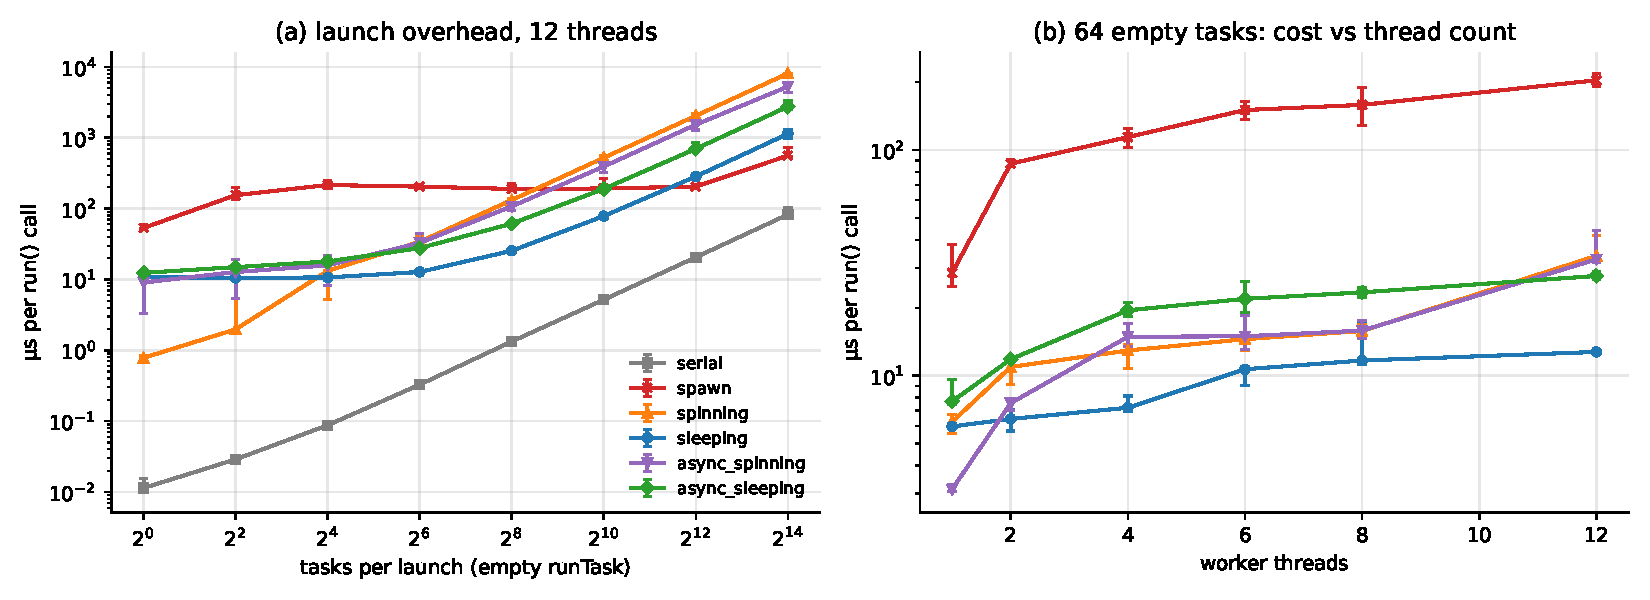
\includegraphics[width=\linewidth]{cpp_launch_overhead.pdf}
\caption{空任务 launch 的开销。(a) 12 线程，横轴为每次 launch 的任务数；(b) 64 个空任务，横轴为线程数。误差棒为 9 次测量的最小--最大值。数据：\texttt{overhead.jsonl}。}
\label{fig:overhead}
\end{figure}

\begin{table}[H]
\centering
\caption{空任务 launch 开销（µs / \texttt{run()}，12 线程）}
\label{tab:overhead}
\small
\begin{tabular}{rrrrrrr}
\toprule
任务数 & serial & spawn & spinning & sleeping & async\_\allowbreak{}spinning & async\_\allowbreak{}sleeping \\
\midrule
1 & 0.0114 & 53.3 & 0.783 & 10.8 & 9.05 & 12.4 \\
16 & 0.0876 & 215 & 13.2 & 10.7 & 15.8 & 17.9 \\
64 & 0.328 & 204 & 34.0 & 12.7 & 32.8 & 27.7 \\
1024 & 5.18 & 192 & 521 & 78.3 & 393 & 190 \\
16384 & 82.3 & 558 & 8100 & 1140 & 5270 & 2750 \\
\bottomrule
\end{tabular}
\end{table}

\Cref{fig:overhead} 与表~\ref{tab:overhead} 可以把 launch 开销拆成三部分：建线程、唤醒和每个任务的分发。

先看建线程。spawn 在 1 个任务时只建 1 个线程，耗时 53.3~µs；64 个任务时建 12 个线程，耗时 204~µs。
\cref{fig:overhead}(b) 中，spawn 从 1 线程的 28.6~µs 线性涨到 12 线程的 204~µs，约每个线程 16~µs（\texttt{clone}、调度和 \texttt{join}）。
这正是常驻线程池要摊掉的成本：同样 64 个空任务，睡眠池只要 12.7~µs，是 spawn 的 1/16。

再看唤醒。1 个任务时，自旋池 0.783~µs，睡眠池 10.8~µs，差 13.8 倍。
自旋池的 worker 一直在读 \texttt{state\_\allowbreak{}}，调用者发布新 generation 后，只需一次 cache line 迁移（约百纳秒级）就能被看到。
睡眠池则要走完一整条路径：\texttt{notify\_\allowbreak{}all} 触发 futex 系统调用，内核再把 worker 调度上核；完成时还要反方向再唤醒一次调用者。两次线程唤醒合计约 10~µs。

最后看每个任务的分发。任务数增大后，曲线的斜率反映的就是每个任务的分发成本。16384 个空任务时，串行 5.0~ns/任务，spawn 34~ns，睡眠池 70~ns，
自旋池却高达 494~ns，async 系统为 168--322~ns。自旋池在 64 个任务以上反而比睡眠池慢，原因是 \emph{竞争}。
12 个自旋 worker 同时对同一个 64 位状态做 CAS，失败的 CAS 要重读重试，所以每次成功认领平均伴随着多次失败。
此外，每个任务都要对 \texttt{done\_\allowbreak{}} 做一次 \texttt{fetch\_\allowbreak{}add}，而调用者正在自旋读同一个（很可能在同一行上的）\texttt{done\_\allowbreak{}}。
睡眠池的 worker 是依次被唤醒的，同一时刻真正在抢的线程更少，冲突反而少。
spawn 用的是不会失败的 \texttt{fetch\_\allowbreak{}add}，也没有 \texttt{done} 计数器（靠 \texttt{join} 等待），所以每任务成本最低。
\cref{sec:dispatch} 的微基准会单独验证这一点。

\begin{findingbox}[：launch 开销]
常驻线程池把每次 launch 的固定开销从 spawn 的约 200~µs 降到 1--13~µs，自旋又把唤醒延迟降了一个数量级（0.783 对 10.8~µs）。
但``自旋最快''只在任务数少时成立：任务一多，CAS 争用让自旋池每任务 494~ns，是睡眠池的 7 倍。
\end{findingbox}

\subsection{Q2：官方测试上谁快？}

知道了开销的构成，就可以预测：任务越小，唤醒和分发越重要；任务越大，这些开销越无所谓。官方 20 个测试正好覆盖了这两端。

\begin{figure}[H]
\centering
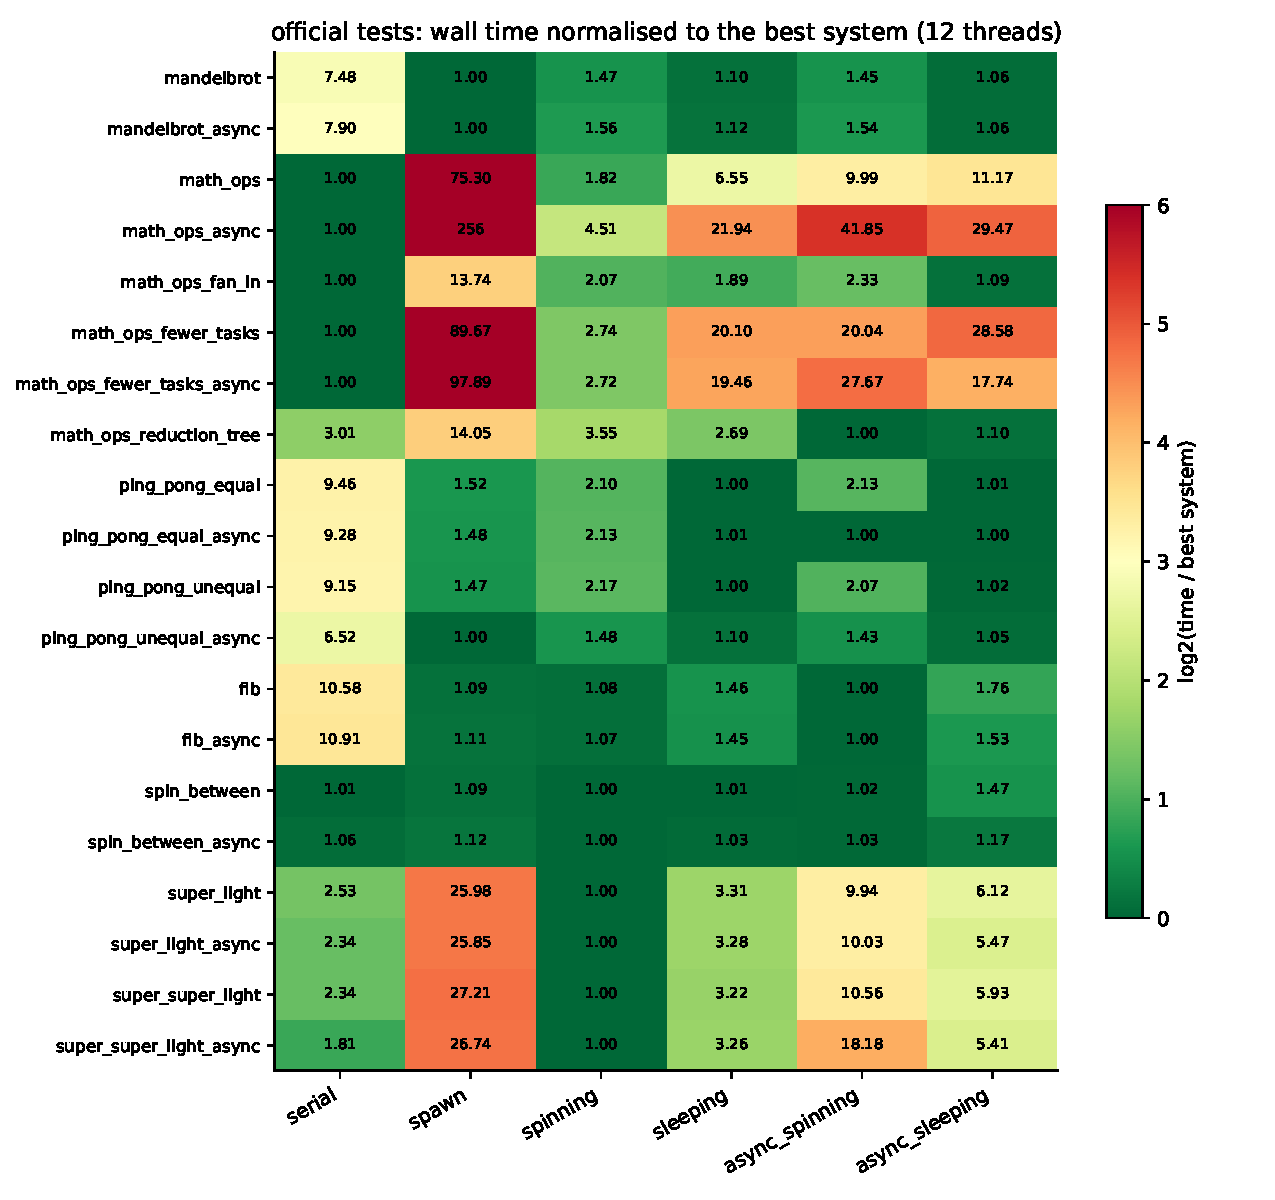
\includegraphics[width=0.86\linewidth]{cpp_test_heatmap.pdf}
\caption{20 个官方测试 × 6 个系统，墙钟时间除以该行最快系统（格内数字），颜色为 $\log_2$。数据：\texttt{tests.jsonl}。}
\label{fig:heatmap}
\end{figure}

\begin{table}[H]
\centering
\caption{部分官方测试的墙钟时间（ms，12 线程）}
\label{tab:tests_ms}
\small
\begin{tabular}{lrrrrrr}
\toprule
测试 & serial & spawn & spinning & sleeping & async\_\allowbreak{}spin & async\_\allowbreak{}sleep \\
\midrule
super\_\allowbreak{}super\_\allowbreak{}light & 7.26 & 84.4 & 3.10 & 9.98 & 32.8 & 18.4 \\
math\_\allowbreak{}ops\_\allowbreak{}in\_\allowbreak{}tight\_\allowbreak{}for\_\allowbreak{}loop & 5.14 & 387 & 9.35 & 33.6 & 51.3 & 57.4 \\
ping\_\allowbreak{}pong\_\allowbreak{}equal & 133 & 21.3 & 29.4 & 14.0 & 29.8 & 14.2 \\
ping\_\allowbreak{}pong\_\allowbreak{}unequal & 143 & 22.9 & 33.8 & 15.6 & 32.3 & 16.0 \\
recursive\_\allowbreak{}fibonacci & 77.1 & 7.95 & 7.90 & 10.7 & 7.29 & 12.8 \\
mandelbrot\_\allowbreak{}chunked & 329 & 44.0 & 64.9 & 48.4 & 64.0 & 46.5 \\
math\_\allowbreak{}ops\_\allowbreak{}fan\_\allowbreak{}in & 25.8 & 354 & 53.4 & 48.8 & 60.0 & 28.0 \\
math\_\allowbreak{}ops\_\allowbreak{}reduction\_\allowbreak{}tree & 23.8 & 111 & 28.1 & 21.3 & 7.91 & 8.70 \\
spin\_\allowbreak{}between\_\allowbreak{}run\_\allowbreak{}calls & 6.36 & 6.87 & 6.28 & 6.37 & 6.39 & 9.22 \\
\bottomrule
\end{tabular}
\end{table}

读\cref{fig:heatmap} 时，可以按``每次 launch 有多少工作''把测试分成三类。

第一类是 launch 开销主导的测试（\texttt{super\_\allowbreak{}super\_\allowbreak{}light}、\texttt{super\_\allowbreak{}light}、\texttt{math\_\allowbreak{}operations\_\allowbreak{}in\_\allowbreak{}tight\_\allowbreak{}for\_\allowbreak{}loop*}）。
每个任务只有约 100~ns 的工作（2048 个元素分给 16 个任务），一次 launch 的有用工作不到 2~µs。
在这里，spawn 比最快的系统慢 26--255 倍；睡眠池也比串行慢（\texttt{math\_\allowbreak{}ops} 上 33.6 对 5.14~ms）；
只有自旋池能接近或胜过串行，\texttt{super\_\allowbreak{}super\_\allowbreak{}light} 上为 3.10~ms，比串行快 2.3 倍。
官方正是用这组测试来检验``线程池是否真的常驻、唤醒是否够快''。

第二类是计算主导的测试（\texttt{ping\_\allowbreak{}pong}、\texttt{fibonacci}、\texttt{mandelbrot}）。每次 launch 有毫秒级的工作，所有并行系统都比串行快 4--11 倍。
spawn 的 200~µs 被摊薄了，在 mandelbrot 上 spawn 甚至是最快的（44.0~ms，7.5 倍）。
自旋池在 ping-pong 与 mandelbrot 上比睡眠池慢约一倍，但问题不在自旋本身：12 个自旋 worker 加上自旋等待的调用者，一共 13 个忙线程挤在 12 个核上，详见\cref{sec:caller}。

第三类是依赖图主导的测试（\texttt{fan\_\allowbreak{}in}、\texttt{reduction\_\allowbreak{}tree}）。同步系统必须一层一层地 launch，每层的尾部都有线程闲着；
async 系统则让不同分支的 launch 同时进入 ready 队列。归约树上 async 为 7.91--8.70~ms，比同步睡眠池（21.3~ms）快 2.4--2.7 倍，也是唯一明显胜过串行（23.8~ms）的系统。

\begin{findingbox}[：没有一个系统在所有测试上最快]
调度器的``最优''取决于任务粒度与图结构：每次 launch 只有几微秒工作时只有自旋池能赢串行，工作到毫秒级时连 spawn 都接近最优，依赖图测试则只有 async 系统能赢。
\end{findingbox}

\subsection{Q3：线程扩展}

上一节只看了 12 线程。把线程数从 1 加到 12，能看到哪些系统扩展得好、在哪里掉队，也会暴露一个我没能完全解释的现象。

\begin{figure}[H]
\centering
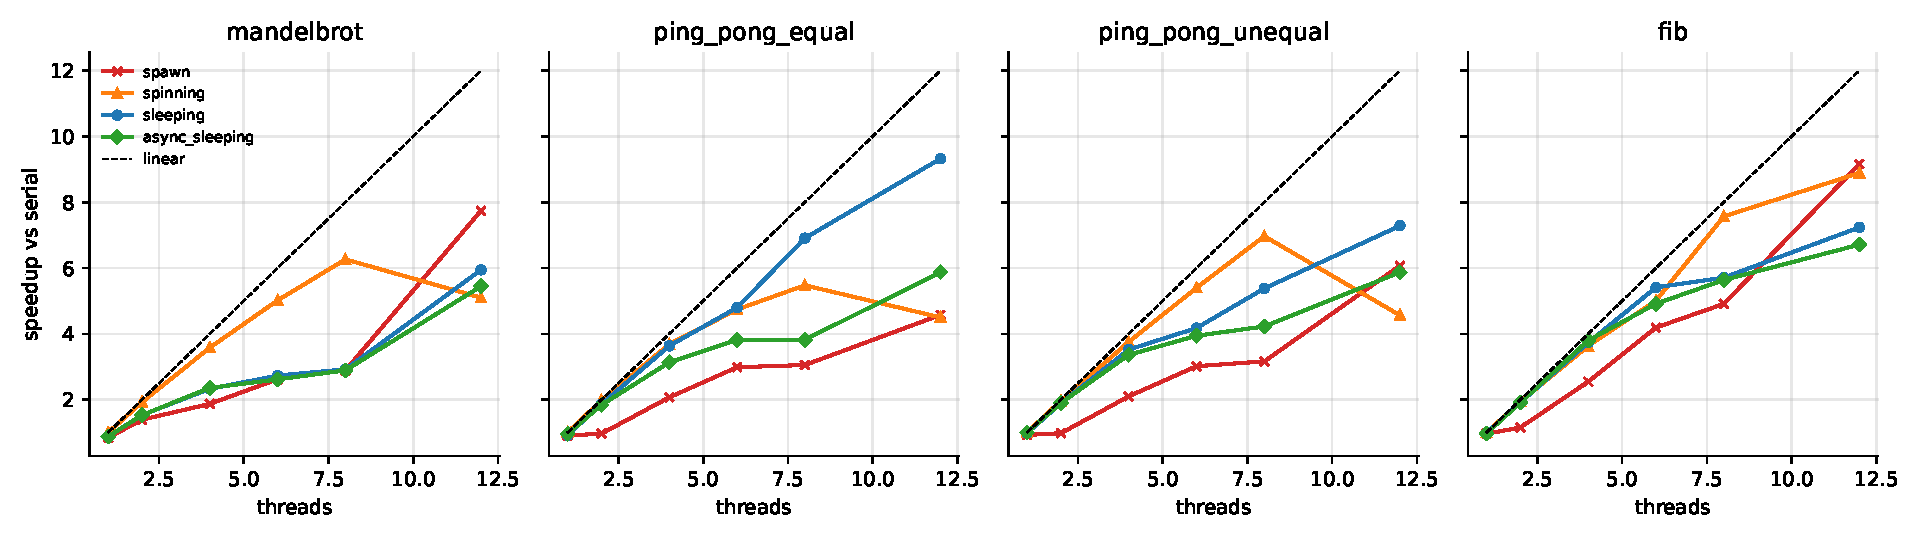
\includegraphics[width=\linewidth]{cpp_thread_scaling.pdf}
\caption{计算主导测试的加速比（相对串行），1--12 线程。数据：\texttt{scaling.jsonl}。}
\label{fig:scaling}
\end{figure}

串行基线是：mandelbrot 332.8~ms、ping\_\allowbreak{}pong\_\allowbreak{}equal 132.0~ms、ping\_\allowbreak{}pong\_\allowbreak{}unequal 145.0~ms、fibonacci 76.5~ms。
\Cref{fig:scaling} 里有三个现象。

其一，1--4 线程时，所有常驻池都接近线性（fibonacci 4 线程 3.6--3.8 倍）。

其二，自旋池在 8 线程时 mandelbrot 为 6.26 倍、ping\_\allowbreak{}pong\_\allowbreak{}unequal 为 6.97 倍，到 12 线程反而降到 5.10 与 4.57 倍（fibonacci 仍从 7.57 升到 8.89 倍）。
这是``调用者也占一个核''的效应：8 线程时调用者还有空闲核可用，12 线程时就没有了。fibonacci 不受影响，是因为它每个 launch 有 256 个约 0.3~ms 的任务，被换下的 worker 只拖慢少数几个任务。

其三，睡眠池在 12 线程时最好（ping\_\allowbreak{}pong\_\allowbreak{}equal 9.33 倍），但 mandelbrot 在 2--8 线程时只有 1.53--2.92 倍，明显低于自旋池；spawn 与 async 睡眠池也是如此。
这一点在 3 轮实验中都复现了。容器里没有 \texttt{perf}/\texttt{turbostat} 权限，所以我只能用已有数据加上一组本机对照，尽量把原因的范围缩小（\cref{fig:anomaly}）。

\begin{figure}[H]
\centering
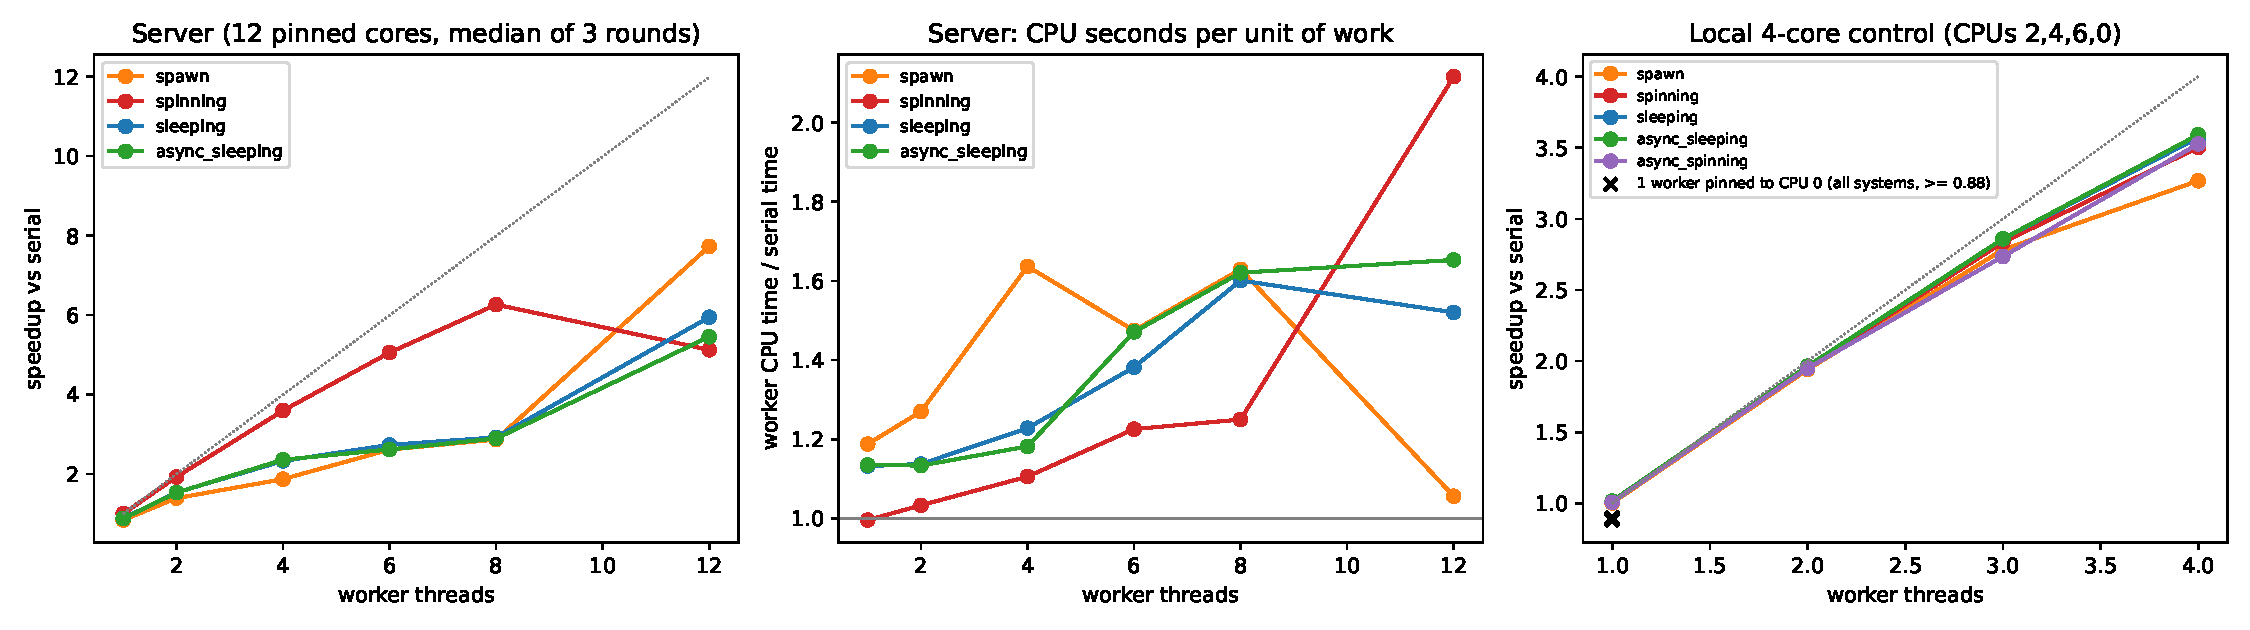
\includegraphics[width=\linewidth]{cpp_mandel_anomaly.pdf}
\caption{mandelbrot\_\allowbreak{}chunked 的扩展缺口。左：服务器加速比（3 轮中位数）。中：服务器上``完成同样工作消耗的 CPU 秒 / 串行秒''，自旋类先减去调用者自旋的一个核。
右：本机 4 核对照（worker 绑在逻辑 CPU 2、4、6、0 上，每个 worker 独占一个物理核），叉号是 1 个 worker 绑在 CPU~0 上。数据：\texttt{scaling.jsonl}、\texttt{local4c/scaling\_\allowbreak{}mandel*.jsonl}；脚本 \texttt{scripts/plot\_\allowbreak{}anomaly.py}。}
\label{fig:anomaly}
\end{figure}

排查分三步。

\begin{enumerate}
\item 1 个 worker 时就已经慢了。同一个核、同一份工作，睡眠池 377\,ms、async 睡眠池 377\,ms、spawn 378--399\,ms，而自旋池是 333\,ms，与串行相同。
唤醒开销每次 launch 只有几到几十微秒，4 次 launch 解释不了 44\,ms 的差距；只有 1 个 worker，也谈不上负载不均。
\item 慢在执行，而不在等待。睡眠池 1 线程的进程 CPU 时间是 377\,ms，等于墙钟，说明 worker 一直在跑，只是同样的指令多花了 13\% 的 CPU 时间。
如果原因是``被唤醒后排队等其他租户让出核''，CPU 时间应当仍是 333\,ms，只有墙钟变长。8 线程时，睡眠类的 CPU 秒 / 串行秒涨到 1.60--1.63，自旋池是 1.25。
\item 这也不是睡眠池设计本身的性质。本机 4 核上，四种常驻池（睡眠、自旋及两个 async 版本）在 1--4 线程的加速比互相差不到 5\%，4 线程时为 3.50--3.59 倍，睡眠池（3.57）还略快于自旋池（3.50）；
只有每次 launch 都新建线程的 spawn 在 4 线程时落后（3.27 倍）。睡眠类的 CPU 秒 / 串行秒恒为 0.98--1.01。
本机唯一的系统性慢化出现在逻辑 CPU~0 上：任何实现（包括自旋池）把 1 个 worker 绑在 CPU~0 上都会慢 11--13\%，与新建线程还是常驻线程、调用者自旋还是睡眠都无关。
\end{enumerate}

所以服务器上的现象可以概括为：进程里有线程在自旋时，worker 跑得快；所有非工作线程都睡下时，worker 的每条指令更贵。
它与 A1 报告中``新建的工作线程比主线程慢''是同一类现象（那里每次 launch 固定多出约 9\,ms，与图像视角无关，是加性而不是乘性的）。
与数据一致的候选解释是宿主机的频率与空闲管理：有线程自旋时，CPU 不进入空闲状态，保持在高频；否则，刚空闲过的核需要重新升频，或者它的 SMT 兄弟被其他租户占用了。
要区分这两个候选需要 \texttt{turbostat}（每核频率、C-state 驻留），本文只能排除``唤醒开销''``负载不均''和``睡眠池实现缺陷''三种解释。
12 线程时 spawn 反而达到 7.73 倍，CPU 秒 / 串行秒回到 1.06，这也说明这个现象取决于测量时宿主机的状态，而不是实现。

\subsection{Q4：自旋与睡眠的 CPU 代价}

到目前为止只比较了墙钟时间。自旋的快不是白来的，这一节把它花掉的 CPU 算出来。

\begin{figure}[H]
\centering
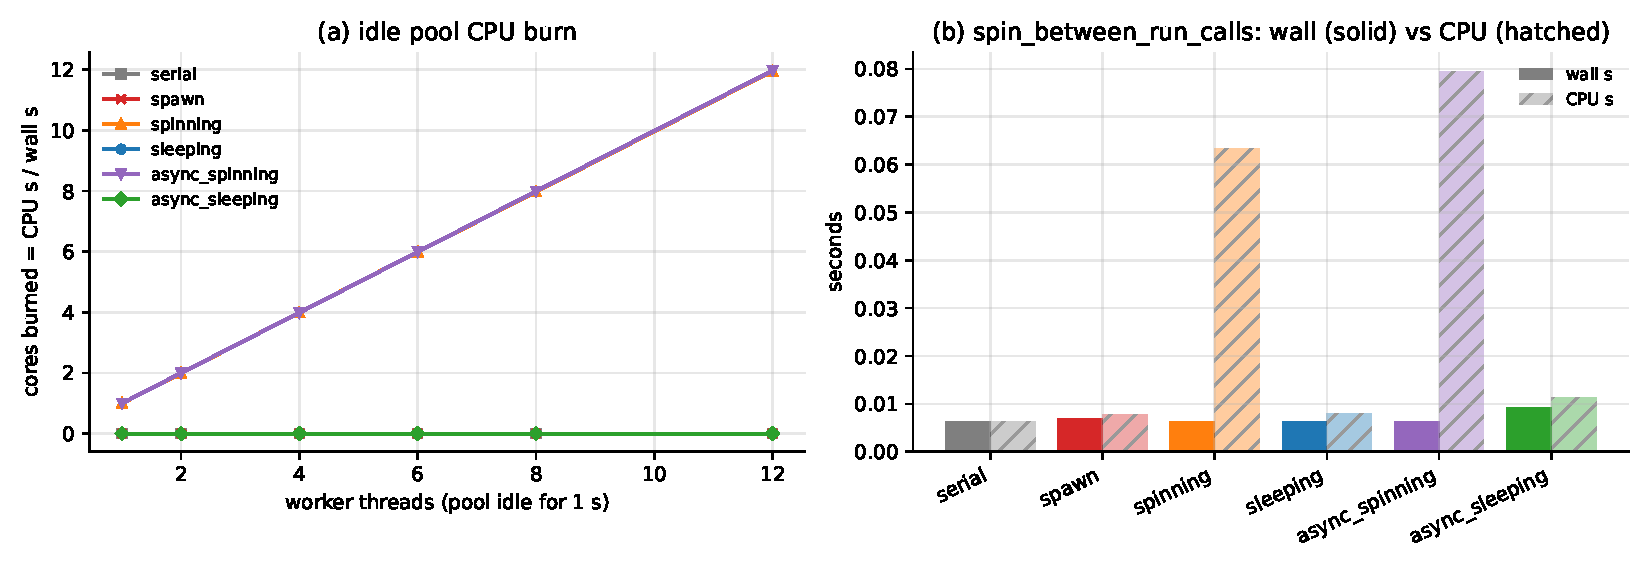
\includegraphics[width=\linewidth]{cpp_idle_cpu_burn.pdf}
\caption{(a) 线程池空闲 1~s 时消耗的核数（进程 CPU 时间 / 墙钟）；(b) \texttt{spin\_\allowbreak{}between\_\allowbreak{}run\_\allowbreak{}calls} 的墙钟与 CPU 时间。数据：\texttt{idle.jsonl}、\texttt{tests.jsonl}。}
\label{fig:idle}
\end{figure}

\begin{figure}[H]
\centering
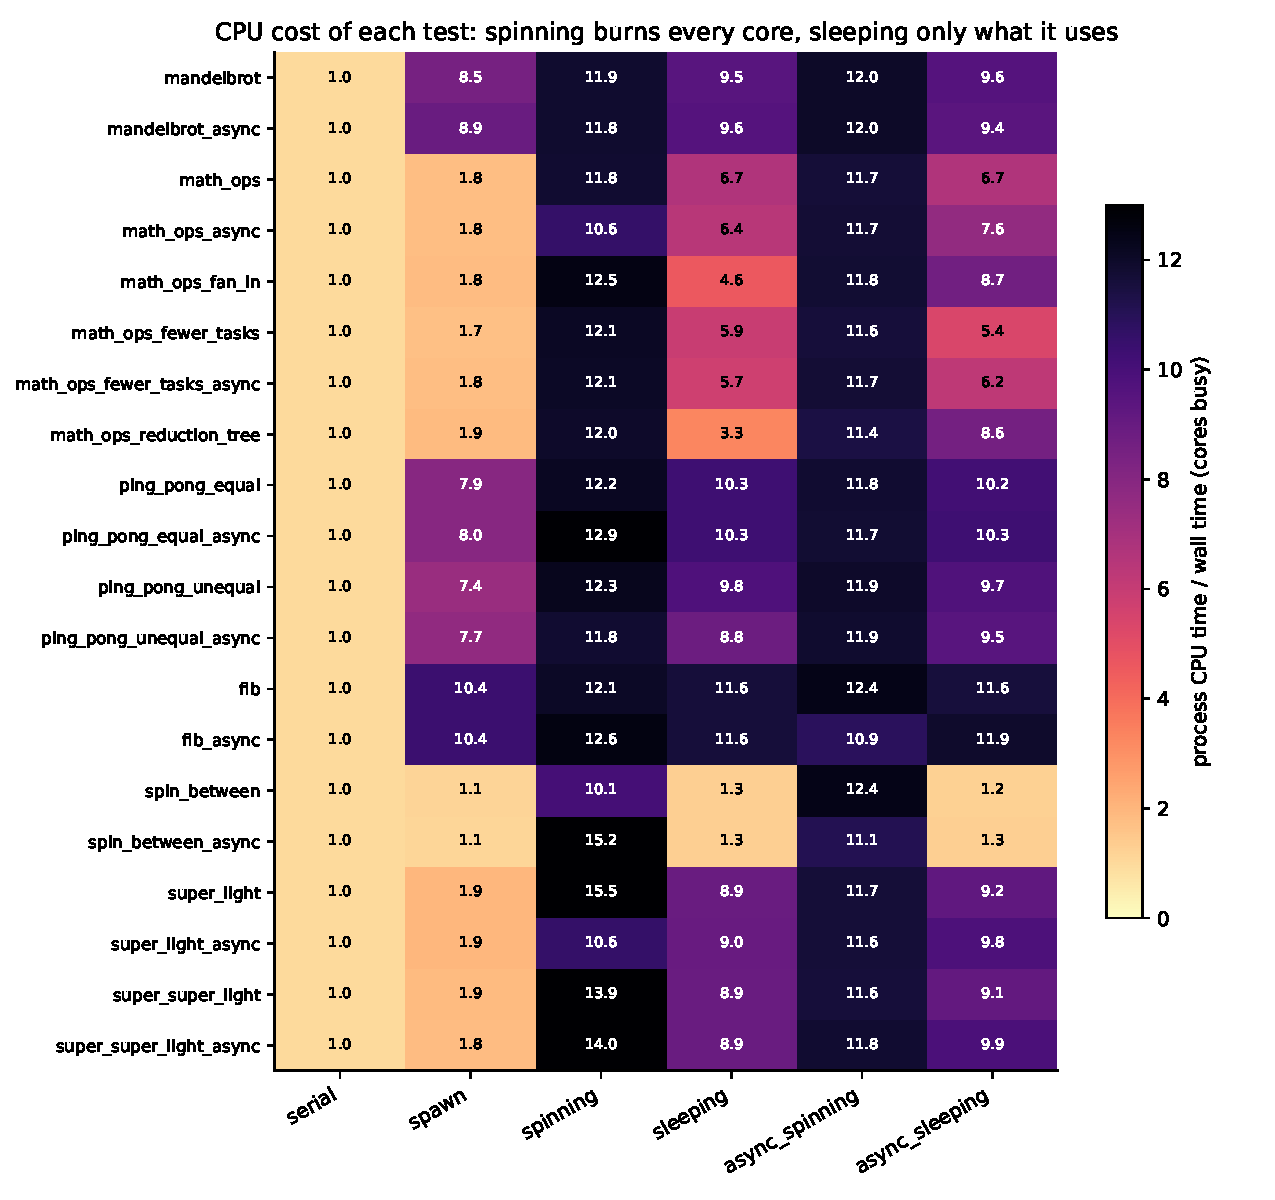
\includegraphics[width=0.86\linewidth]{cpp_test_cpu_cost.pdf}
\caption{每个官方测试的 CPU 时间 / 墙钟时间（平均忙碌的核数）。数据：\texttt{tests.jsonl} 的 \texttt{cpu\_\allowbreak{}s}。}
\label{fig:cpucost}
\end{figure}

线程池空闲 1~s 时，自旋池消耗的核数严格等于线程数（12 线程 11.96 核），睡眠池为 0.00（\cref{fig:idle}a）。

\texttt{spin\_\allowbreak{}between\_\allowbreak{}run\_\allowbreak{}calls} 更有代表性：调用者在两次 launch 之间串行计算 fib(27)，这段时间 worker 无事可做。
自旋池墙钟 6.28~ms、CPU/墙钟 10.09；睡眠池墙钟 6.37~ms、CPU/墙钟 1.27。墙钟几乎相同，是因为本实验里每个 worker 独占一个核，
自旋浪费掉的只是``别人本可以用''的 CPU。一旦线程数超过核数（\cref{sec:oversub}），或者机器上有其他进程，这些 CPU 就会直接变成别人的延迟。

\cref{fig:cpucost} 展示了同一现象的全貌。自旋类系统在每个测试上都在烧 10--15 个核（超过 12 是因为调用者也在自旋）；
睡眠池只在计算主导的测试上接近 10 个核，在 \texttt{math\_\allowbreak{}ops} 这种 launch 主导的测试上只有 3--7 个核。
在空任务 launch 循环（64 任务）中，自旋池 CPU/墙钟为 12.0，睡眠池 7.09，spawn 1.82。

\begin{findingbox}[：自旋的真实代价]
自旋是用 CPU 换延迟：在 12 个独占核上，它把唤醒延迟从 10.8~µs 降到 0.783~µs，代价是空闲时也烧满 12 个核。
在共享机器、容器配额或电池供电的设备上，这些 CPU 不是免费的。
\end{findingbox}

\subsection{Q5：超额订阅（线程数多于核数）}
\label{sec:oversub}

上一节说到，自旋浪费的 CPU 在线程数超过核数时会变成别人的延迟。超额订阅实验就是把这种情况直接制造出来，看各系统能退化到什么程度。

\begin{figure}[H]
\centering
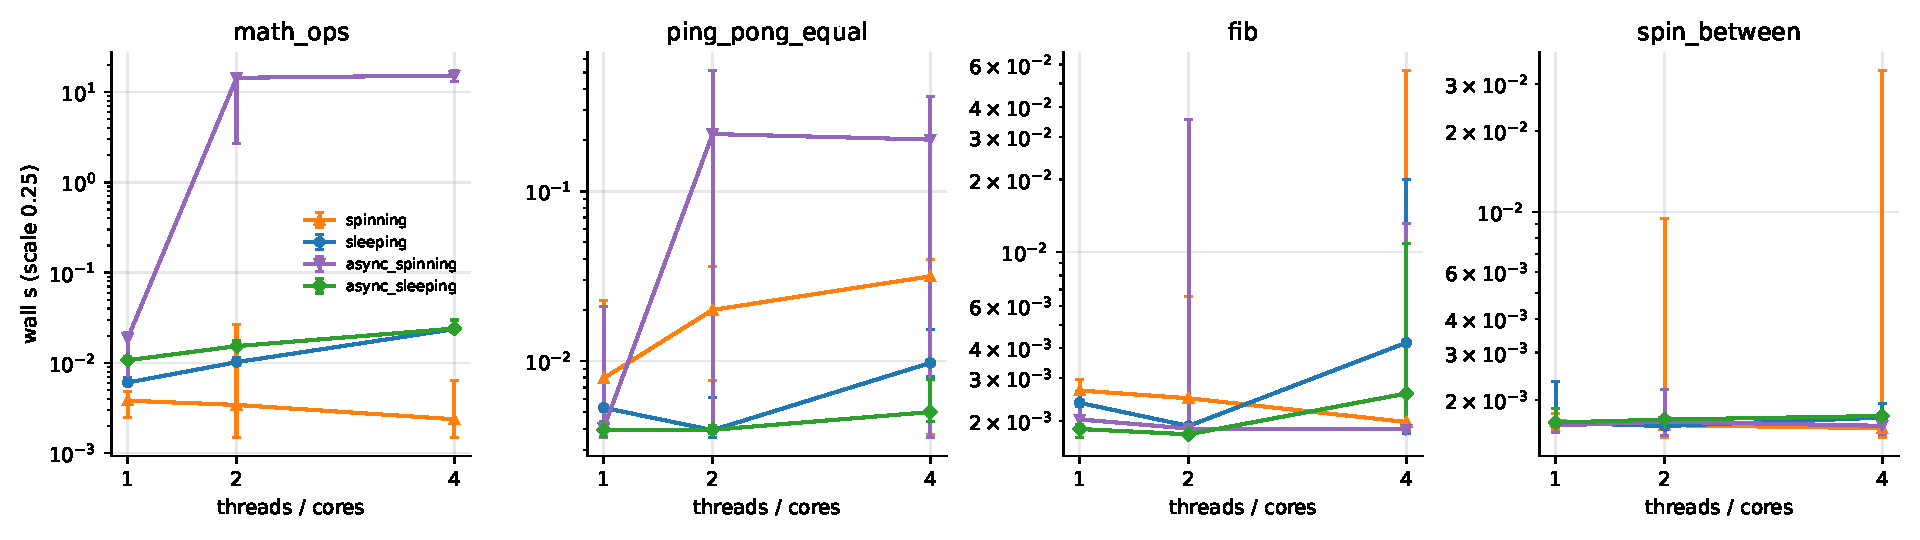
\includegraphics[width=\linewidth]{cpp_oversubscription.pdf}
\caption{12 个核上运行 12、24、48 个 worker（规模 0.25）。纵轴对数。数据：\texttt{oversub.jsonl}。}
\label{fig:oversub}
\end{figure}

\begin{table}[H]
\centering
\caption{超额订阅下的墙钟时间（ms，规模 0.25）}
\label{tab:oversub}
\small
\begin{tabular}{llrrrr}
\toprule
测试 & 线程/核 & spinning & sleeping & async\_\allowbreak{}spinning & async\_\allowbreak{}sleeping \\
\midrule
math\_\allowbreak{}ops & 1× & 3.81 & 6.06 & 18.8 & 10.7 \\
 & 2× & 3.42 & 10.2 & 14400 & 15.3 \\
 & 4× & 2.37 & 23.7 & 15300 & 24.0 \\
ping\_\allowbreak{}pong\_\allowbreak{}equal & 1× & 7.93 & 5.32 & 4.03 & 3.95 \\
 & 2× & 20.0 & 3.92 & 217 & 3.94 \\
 & 4× & 31.6 & 9.76 & 201 & 5.02 \\
\bottomrule
\end{tabular}
\end{table}

\Cref{fig:oversub} 与表~\ref{tab:oversub} 中最醒目的是 async\_\allowbreak{}spinning：2 倍超额订阅时，\texttt{math\_\allowbreak{}ops} 从 18.8~ms 变成 14400~ms（约 766 倍），
CPU 时间 173~s。原因是 \emph{锁持有者被抢占}（lock-holder preemption）。
Part~B 的 spinning 版用一把互斥锁保护 ready 队列。24 个线程里，持锁的那个一旦被内核换下，其余线程要么在自旋读 \texttt{ready\_\allowbreak{}count\_\allowbreak{}}，把持锁者急需的 CPU 时间片烧掉，要么在锁上排队；
于是每次 launch 都可能要付一个调度时间片（毫秒级）。

Part~A 的自旋池没有锁（用 CAS 认领），所以 \texttt{math\_\allowbreak{}ops} 在 4 倍超额订阅时仍只要 2.37~ms。
但 ping-pong 每个任务约 0.2~ms，认领了任务的 worker 被抢占时，整个 launch 都要等它回来，所以自旋池从 7.93 涨到 31.6~ms。
睡眠类系统在 2 倍时几乎不受影响（async\_\allowbreak{}sleeping 3.94~ms），到 4 倍时才因为要唤醒更多线程而开始变慢。

\begin{findingbox}[：超额订阅]
自旋只在``线程数 $\le$ 空闲核数''时划算；自旋、加锁、超额订阅凑在一起是最坏的组合（766 倍变慢）。
生产级运行时（TBB、OpenMP 的 \texttt{OMP\_\allowbreak{}WAIT\_\allowbreak{}POLICY}）因此都采用``先自旋一小段，再 yield，再睡眠''的混合等待策略~\cite{tbb}，这一思想可追溯到 Ousterhout 的 spin-then-block~\cite{ousterhout}。
\end{findingbox}

\subsection{Q6：任务粒度}

把同样多的工作切成多少个任务最合适？切得太粗，负载不均；切得太细，分发开销占上风。这一节用一条粒度曲线把两头都画出来。

\begin{figure}[H]
\centering
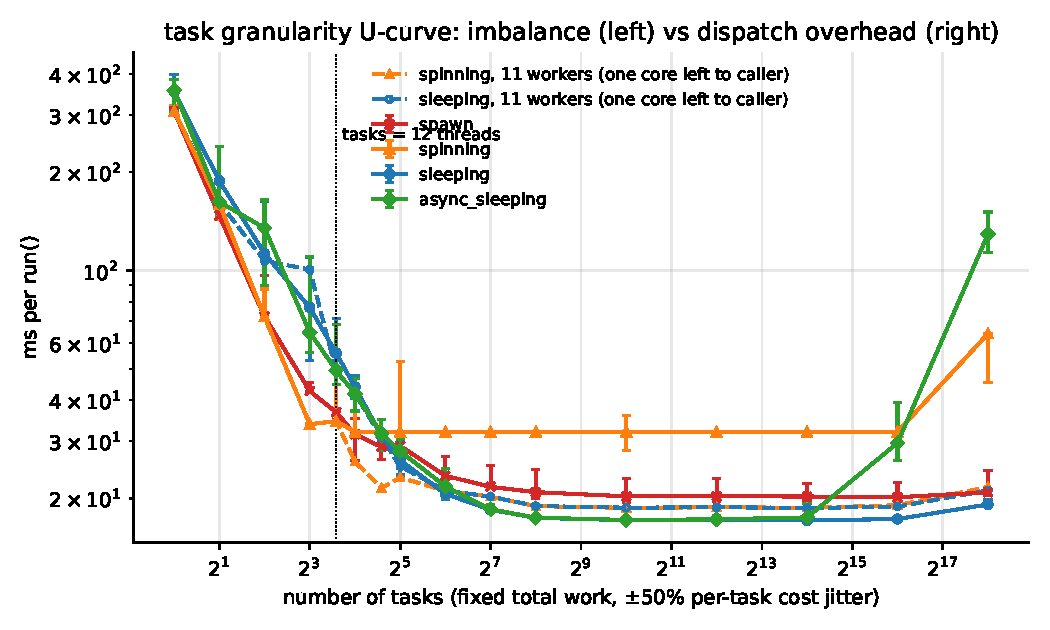
\includegraphics[width=0.85\linewidth]{cpp_granularity.pdf}
\caption{固定总工作量（$2\times10^8$ 次 LCG 迭代），切成 1--262144 个任务，每个任务代价乘以 $[0.5,1.5]$ 内的随机系数。虚线为 11 个 worker 的对照。数据：\texttt{granularity.jsonl}、\texttt{granularity\_\allowbreak{}11workers.jsonl}。}
\label{fig:gran}
\end{figure}

由 DAG 实验的串行基线（\cref{sec:dag}）可以算出每次 LCG 迭代 1.03~ns，所以总工作量串行约 206~ms，12 线程的理想值约 17.1~ms。
\Cref{fig:gran} 是经典的 U 形曲线。

曲线左侧是任务太少的情形。12 个任务时睡眠池要 55.8~ms，因为每个线程只有一个任务，无法均衡，最慢的任务决定完成时间。
任务数增加到 256 以上时，动态分配把 $\pm 50\%$ 的抖动平均掉了，睡眠池稳定在 17.1--17.5~ms，即理想值的约 100\%。

曲线右侧是任务太多的情形。async\_\allowbreak{}sleeping 每个任务都要进一次全局锁，65536 个任务时 29.6~ms，262144 个任务时 129~ms（约 490~ns/任务，这是锁造成的串行化）。
睡眠池在 262144 个任务时只到 19.2~ms；spawn 从 256 个任务起一直保持在 20.2--20.9~ms，因为 \texttt{fetch\_\allowbreak{}add} 不会失败。

自旋池的曲线形状很特别。12 个 worker 时，它从 24 个任务开始固定在 32.0~ms，262144 个任务时恰好翻倍到 64.0~ms。
这种``量子化''的时间是调度时间片的特征：调用者线程与某个 worker 分时共享一个核，被换下的 worker 手里的任务要等一个时间片才能继续。
改用 11 个 worker 后（虚线），自旋池在 1024 个任务时为 18.7~ms，平台消失了。

\subsection{调用者线程占不占核；SMT}
\label{sec:caller}

前面几节已经三次碰到``调用者占核''的影子：自旋池在 12 线程时扩展变差、ping-pong 上比睡眠池慢一倍、粒度曲线上出现 32.0~ms 的平台。
这一节直接比较 12 个 worker 和 11 个 worker，再顺便看看把 SMT 兄弟核也用上会怎样。

\begin{figure}[H]
\centering
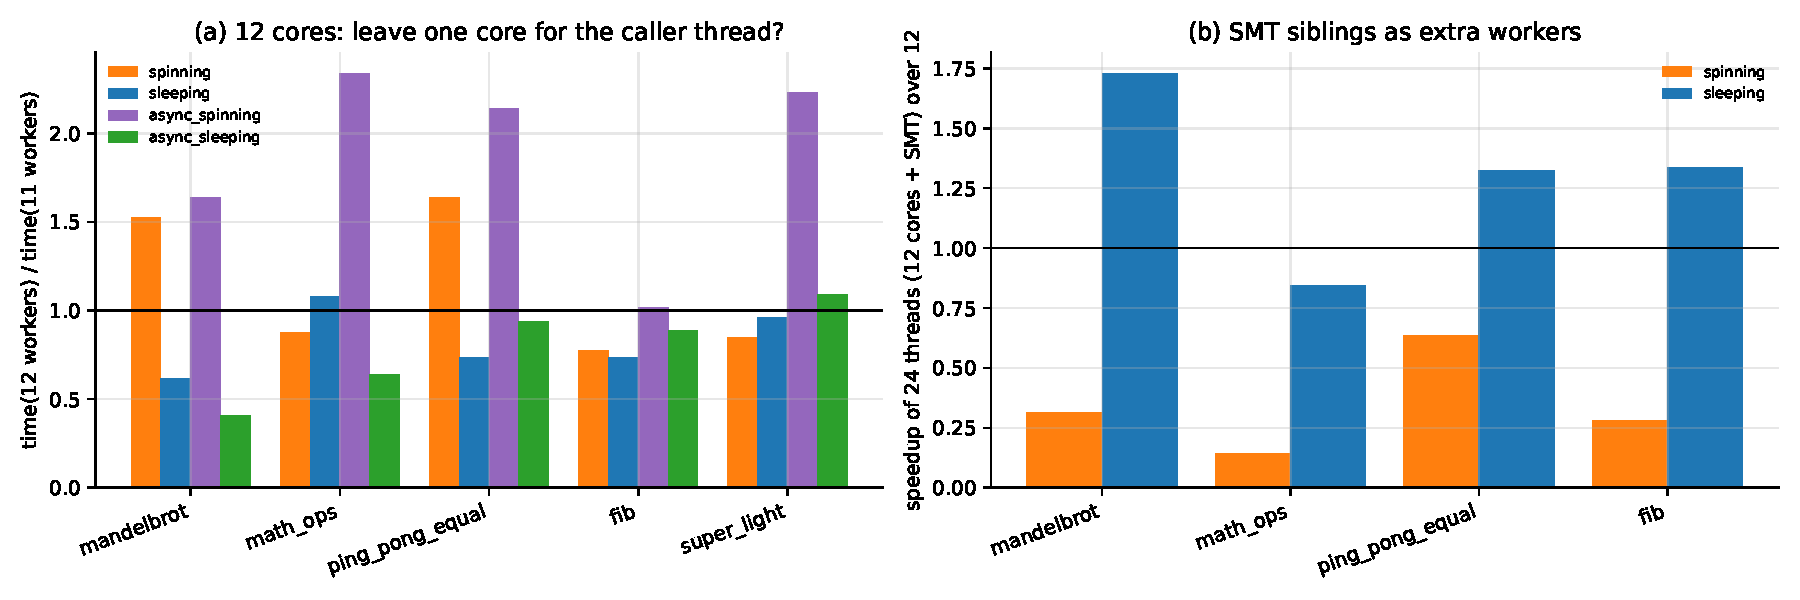
\includegraphics[width=\linewidth]{cpp_caller_smt.pdf}
\caption{(a) 12 个核上用 12 个 worker 与 11 个 worker 的时间比（$>1$ 表示留一个核给调用者更好）；(b) 12 个物理核上用 24 个 worker（加 SMT 兄弟核）相对 12 个 worker 的加速。单轮 3 次测量。数据：\texttt{caller\_\allowbreak{}core.jsonl}、\texttt{smt.jsonl}。}
\label{fig:caller}
\end{figure}

\Cref{fig:caller}(a) 显示，对自旋池来说，11 个 worker 比 12 个更快：ping\_\allowbreak{}pong\_\allowbreak{}equal 为 19.7 对 32.3~ms，mandelbrot 为 42.1 对 64.2~ms；
async\_\allowbreak{}spinning 同样如此（ping\_\allowbreak{}pong 13.9 对 29.7~ms）。
睡眠类系统的调用者在等待时会睡下，不需要独占一个核；这组数据只有一轮，噪声较大（例如 async\_\allowbreak{}sleeping mandelbrot 92.7 对 37.6~ms），所以不下结论。
由此得到一条实用规则：\textbf{自旋池的 worker 数应设为``可用核数 $-$ 1''，或者让调用者也参与执行任务}（TBB 与 Cilk 的调用者都会参与）。

\Cref{fig:caller}(b) 是 SMT 实验。在 12 个物理核上加入 SMT 兄弟核（24 个 worker）后，睡眠池的 mandelbrot 从 57.9 降到 33.5~ms（1.73 倍），fibonacci 快 1.34 倍，ping-pong 快 1.33 倍。
这些内核受依赖链延迟限制，另一个硬件线程能填满空闲的发射槽~\cite{tullsen}。而 launch 主导的 \texttt{math\_\allowbreak{}ops} 反而变慢（42.9 → 50.9~ms）。
自旋池用 24 个 worker 时则全部变慢（mandelbrot 40.0 → 128~ms、fibonacci 8.64 → 30.6~ms）：自旋的兄弟线程与干活的线程争抢同一个物理核的发射槽，
\texttt{pause} 只能缓解，不能消除。

\subsection{Q7：异步 DAG 与 work/span}
\label{sec:dag}

Part~B 的 \texttt{runAsyncWithDeps} 到底能带来多少收益？这一节先用 6 种依赖形状测出 async 相对同步的提升，再改变每个 launch 的任务数，看``填尾''的效果怎样随之变化。

\begin{figure}[H]
\centering
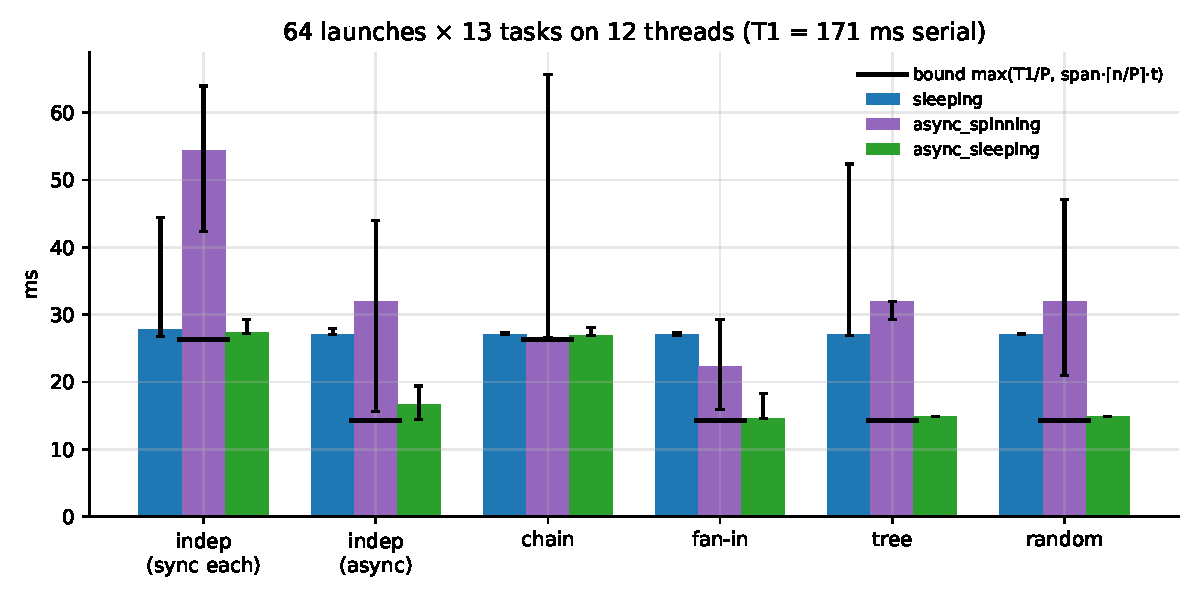
\includegraphics[width=0.85\linewidth]{cpp_dag_shapes.pdf}
\caption{64 个 launch × 13 个任务、每任务 $2\times10^5$ 次迭代，6 种依赖形状。黑线为下界 $\max(T_1/P,\ \text{span}\cdot\lceil n/P\rceil\cdot t)$。数据：\texttt{dag.jsonl}。}
\label{fig:dag}
\end{figure}

\begin{figure}[H]
\centering
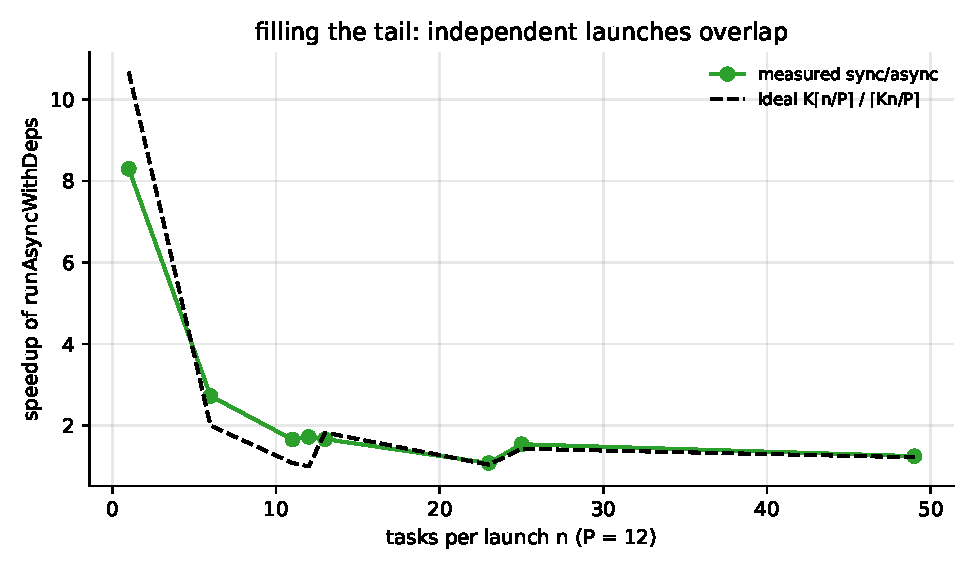
\includegraphics[width=0.7\linewidth]{cpp_async_tail.pdf}
\caption{64 个独立 launch：每次 launch 后同步与全部 async 提交后一次 \texttt{sync} 的时间比，随每 launch 任务数 $n$ 变化（$P=12$）。数据：\texttt{dag\_\allowbreak{}tasks.jsonl}。}
\label{fig:tail}
\end{figure}

串行执行全部 832 个任务需要 $T_1 = 171$~ms，单个任务 $t = 0.2055$~ms。
13 个任务放在 12 个线程上，正好是尾部浪费最严重的情形：同步执行每个 launch 都需要 2 轮，而第二轮只有 1 个线程在干活。\cref{fig:dag} 的结果如下：
\begin{itemize}
\item 独立 launch：每次同步要 27.3~ms，async 为 16.6~ms，快 1.64 倍；理想比值是 $64\cdot\lceil 13/12\rceil / \lceil 64\cdot13/12\rceil = 128/70 = 1.83$。
\item 链：span（关键路径上的 launch 数）为 64 个 launch，async 为 26.9~ms，与同步相同；下界是 $64\times2\times t = 26.3$~ms，达到 98\%。链上没有可以并行的分支，async 也无能为力。
\item 树、fan-in、随机：span 分别为 7、2、8 个 launch，async\_\allowbreak{}sleeping 都在 14.6--14.8~ms，接近 work 下界 $T_1/P = 14.25$~ms（96\%）。
\item 同步睡眠池对所有形状都是约 27.1~ms：它把每个 launch 当成一道屏障，完全没有利用图的形状。
\item async\_\allowbreak{}spinning 在独立、树、随机三种形状上停在 32.0~ms，与\cref{sec:caller} 的时间片平台相同，原因是 \texttt{sync()} 中自旋的调用者占掉了一个 worker 的核。
\end{itemize}

\Cref{fig:tail} 改变每个 launch 的任务数。$n=1$ 时 async 快 8.3 倍（理想值 $64/\lceil 64/12\rceil = 10.7$）；$n=23$ 时快 1.08 倍（理想 1.04）；$n=25$ 时快 1.54 倍（理想 1.43）。
有意思的是 $n=12$：理想值是 1，因为每个 launch 正好一轮，没有尾部可填，但实测仍有 1.72 倍。
原因是同步执行时，每个 launch 都要等 12 个 worker 中最慢的那个被唤醒并完成，在共享机器上这个``最大值''远大于平均值；
async 让下一个 launch 的任务去填补这段等待，掩盖了这类掉队者（straggler）。

\begin{findingbox}[：异步依赖图]
\texttt{runAsyncWithDeps} 的收益来自两点：填满每个 launch 的尾部（理想加速 $K\lceil n/P\rceil/\lceil Kn/P\rceil$），以及让不相关的分支并行。
树形归约在 12 线程上达到 work 下界的 96\%，同步版本则被逐层屏障卡在 27.1~ms，慢 1.83 倍。
\end{findingbox}

\subsection{Q8：false sharing}

前面多次把开销归到``一个被所有核争抢的 cache line''上。这一节和下一节用微基准直接测量这种争用。
先看 false sharing：不同线程写的是不同变量，但它们恰好落在同一个 64~B 缓存行里。

\begin{figure}[H]
\centering
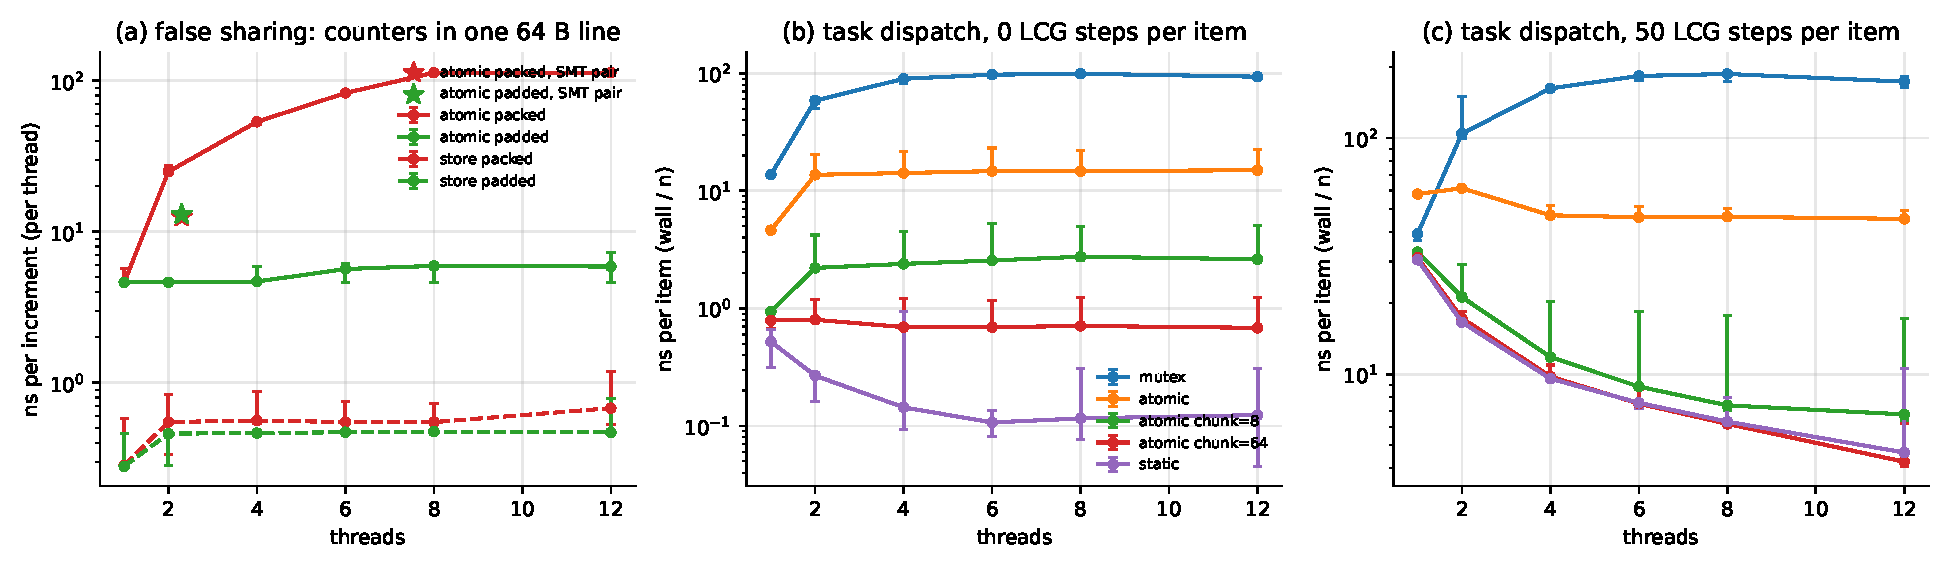
\includegraphics[width=\linewidth]{cpp_contention.pdf}
\caption{(a) 每线程一个计数器：同一 64~B 行内（packed，8~B 步长）与各占一行（padded，64~B 步长）；实线为 \texttt{atomic fetch\_\allowbreak{}add}，虚线为 \texttt{volatile} 读改写；星号为两个线程放在同一物理核的 SMT 兄弟上。
(b)(c) 任务分发计数器：互斥锁、原子 \texttt{fetch\_\allowbreak{}add}、按块 \texttt{fetch\_\allowbreak{}add}（8/64）、静态划分，每项 0 或 50 次 LCG 迭代。数据：\texttt{false\_\allowbreak{}sharing.jsonl}、\texttt{dispatch.jsonl}。}
\label{fig:contention}
\end{figure}

两种布局运行的是完全相同的代码（指针指向同一块 64~B 对齐的缓冲区，只有步长不同），所以单线程时两者一样快（atomic 4.62 对 4.63~ns）。多线程时则差别很大：
\begin{itemize}
\item 原子读改写：packed 在 2 线程时为 25.0~ns，12 线程时 113~ns；padded 始终在 4.63--5.94~ns。12 线程时差 19 倍。
\texttt{lock add} 必须以 Modified 状态独占 cache line，8 个计数器共享一行时，这一行就在 12 个核之间来回迁移（每次约几十纳秒），实际上把 12 个线程串行化了。
\item 普通 \texttt{volatile} 读改写：只差约 1.2--1.4 倍（12 线程 0.679 对 0.470~ns）。一个可能的解释是 store buffer：读操作直接从本核的 store buffer 转发，
写入可以在后台批量提交，不在关键路径上。这一点本文没有用性能计数器验证。
\item SMT 兄弟：两个线程在同一个物理核上时，atomic 版本 packed 与 padded 相同（12.6 对 13.0~ns），因为它们共享 L1，不存在跨核的一致性流量；
但 \texttt{volatile} 版本 packed 是 padded 的 3.4 倍（4.22 对 1.23~ns），推测是同核另一线程写同一行触发了内存序冲突（memory ordering machine clear）。
\end{itemize}

这个微基准我第一次就测错了。第一版把 packed 计数器放在栈数组里，padded 放在 \texttt{alignas(64)} 结构体里，两者生成的地址计算代码不同，
单线程就差了 6.7 倍（1.88 对 0.28~ns），完全掩盖了 false sharing。原始数据保留在 \texttt{false\_\allowbreak{}sharing\_\allowbreak{}v1\_\allowbreak{}confounded.jsonl}。
教训是：\emph{对照组必须只改一个变量}。

\subsection{Q9：任务分发计数器}
\label{sec:dispatch}

动态调度离不开一个共享的分发计数器，它本身就是一个被所有核争抢的 cache line。这一节比较 4 种分发方式，看这个计数器在什么时候会成为瓶颈。

\Cref{fig:contention}(b)(c) 共分发 $10^7$ 个下标。
先看不做任何工作的情形（b）。12 线程下，互斥锁 93.5~ns/项，原子 \texttt{fetch\_\allowbreak{}add} 15.0~ns，每次取 8 个 2.62~ns，每次取 64 个 0.683~ns，静态划分 0.124~ns。
互斥锁比原子慢 6.2 倍，因为锁的获取和释放各是一次原子操作，竞争失败后还有 futex 睡眠与唤醒。
单个原子计数器的吞吐停在约 15~ns/项，与线程数无关，这正是 cache line 在核间迁移一次的时间。换句话说，它是一个 \emph{全局串行点}。

再看每项有 50 次迭代（约 30~ns 工作）的情形（c）。原子计数器在 12 线程时只到 45.5~ns/项（单线程 58.0~ns），几乎不扩展；
按 64 个一块取任务则达到 4.26~ns/项，与静态划分（4.66~ns）相同，加速约 7.3 倍。

这说明了两件事。第一，每个任务的工作量必须远大于约 15~ns 的计数器迁移时间，否则动态调度本身就是瓶颈。
第二，按块取任务（TBB 的 \texttt{grain\_\allowbreak{}size}、OpenMP 的 \texttt{schedule(dynamic, chunk)}）是把争用降低一个块大小倍的最简单办法。
这也解释了\cref{sec:overhead} 中自旋池每个空任务 494~ns 的来源：它用的 CAS 比 \texttt{fetch\_\allowbreak{}add} 更差，失败了就要重试。

%====================================================================
\section{与理论模型的对照}
\label{sec:theory}

上一节的结果是一个个实验测出来的。这一节用几个简单的模型把它们串起来：一个 launch 时间模型、Brent 的 work/span 界、尾部效应公式，以及缓存一致性的串行化模型。
有了这些模型，就能在动手之前估计一个调度器大概能跑多快。

\subsection{launch 时间模型}

把一次 bulk launch 的时间写成
\begin{equation}
T(n, P) = T_{\text{wake}} + \Big\lceil \frac{n}{P} \Big\rceil t_{\text{task}} + n\, t_{\text{disp}}(P) + T_{\text{done}},
\label{eq:launch}
\end{equation}
其中 $T_{\text{wake}}$ 是让 worker 开始干活的时间（spawn 为建线程，约 16~µs/线程；睡眠池约 10~µs；自旋池 $<1$~µs）。
$t_{\text{disp}}(P)$ 是每个任务的分发成本，它随线程数增长，因为分发计数器是一个被 $P$ 个核争抢的 cache line。
空任务实验直接给出了 $t_{\text{disp}}$：睡眠池 70~ns，自旋池 494~ns（16384 任务、12 线程）。

\cref{eq:launch} 给出了任务粒度的下限：要让分发开销低于 10\%，需要 $t_{\text{task}} \ge 10\,P\,t_{\text{disp}}$。
对睡眠池（12 线程），这个下限约为 8~µs；对单个原子计数器的分发（15~ns），约为 2~µs。
\texttt{math\_\allowbreak{}ops} 的任务只有约 100~ns，远低于这个下限，所以所有并行系统都输给了串行。

\subsection{Work/span 与 Brent 定理}

设 DAG 的总工作量为 $T_1$（work），关键路径长度为 $T_\infty$（span）。任意贪心调度器（只要有就绪任务就不让线程闲着）都满足 Brent/Graham 界~\cite{brent,graham}：
\begin{equation}
\max\Big(\frac{T_1}{P},\ T_\infty\Big) \le T_P \le \frac{T_1}{P} + T_\infty .
\label{eq:brent}
\end{equation}
在本文的 launch 级 DAG 中，一个 launch 内的任务彼此独立，所以 $T_\infty = \text{span}\cdot t$（每个 launch 至少要一个任务时间）；
而在``每个 launch 都是屏障''的同步执行下，实际的关键路径变成 $K\lceil n/P\rceil t$。

以树形 DAG（64 个 launch，span 7）为例：$T_1/P = 14.25$~ms，$T_\infty = 7 \times 0.2055 = 1.44$~ms，上界 15.7~ms，实测 14.8~ms，落在 \cref{eq:brent} 的区间内；
同步执行则为 $64\times2\times0.2055 = 26.3$~ms，实测 27.1~ms。
Blumofe 与 Leiserson~\cite{blumofe} 证明了 work stealing 的期望时间为 $T_1/P + O(T_\infty)$（Cilk-5~\cite{cilk5} 与 Chase--Lev deque~\cite{chaselev} 是它的工程实现）。
本文的全局 ready 队列在 12 线程上也达到了这一形式，但代价是每个任务都要进一次全局锁（粒度实验中 262144 个任务时 129~ms）。

\subsection{尾部效应}

$K$ 个各含 $n$ 个任务的独立 launch，同步执行需要 $K\lceil n/P\rceil$ 轮，async 只需 $\lceil Kn/P \rceil$ 轮，所以理想加速为
\begin{equation}
S_{\text{async}} = \frac{K \lceil n/P \rceil}{\lceil Kn/P \rceil}.
\label{eq:tail}
\end{equation}
它在 $n = mP+1$ 时最大（$n=13$ 时为 1.83），在 $n = mP$ 时为 1。\cref{fig:tail} 的实测值在 $n > P$ 时与 \cref{eq:tail} 相差不到 10\%；
$n \le P$ 时实测值高于理论值，因为模型没有计入每个同步 launch 的唤醒与掉队者开销（式~\eqref{eq:launch} 中的 $T_{\text{wake}}+T_{\text{done}}$）。

\subsection{缓存一致性的代价}

在 MESI 类缓存一致性协议下，写一个缓存行之前，要先让其他核上的副本失效。$P$ 个核轮流写同一行时，每次写都需要一次跨核的行迁移，
所以吞吐上限约为 $1/t_{\text{xfer}}$，与 $P$ 无关。实测单个原子计数器在 2--12 线程都是约 14--15~ns/次；
packed 原子计数器 12 线程时每个线程每次 113~ns（总吞吐 $12/113 \approx 0.106$~次/ns，约 9.4~ns/次），量级一致。
Drepper~\cite{drepper} 与 Herlihy \& Shavit~\cite{herlihy} 都把这一点作为``共享计数器不可扩展''的核心论据，Torrellas 等~\cite{torrellas} 最早系统地量化了 false sharing。
Anderson~\cite{anderson} 比较了自旋锁的各种退避策略；MCS 锁~\cite{mcs} 则让每个等待者在自己的 cache line 上自旋，把一致性流量从 $O(P)$ 降到 $O(1)$。

%====================================================================
\section{仓库原有 Python 版本的回顾}
\label{sec:python}

仓库里原有的 Python 版本还有没有价值？把它和 C++ 版放在一起比较，可以看清哪些结论属于调度算法本身，哪些属于执行环境。

\begin{figure}[H]
\centering
\begin{subfigure}{0.49\linewidth}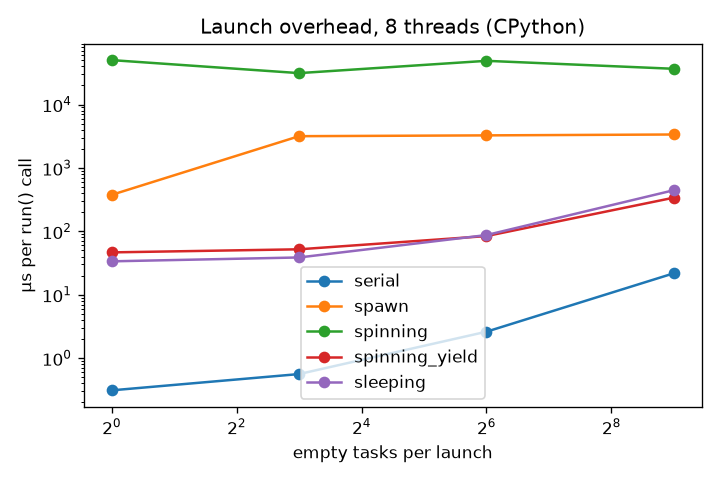
\includegraphics[width=\linewidth]{launch_overhead.png}\caption{launch 开销}\end{subfigure}
\begin{subfigure}{0.49\linewidth}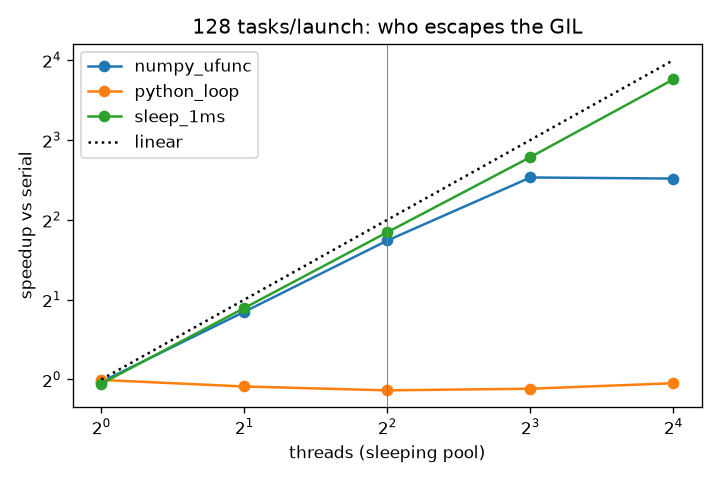
\includegraphics[width=\linewidth]{throughput.png}\caption{吞吐}\end{subfigure}
\begin{subfigure}{0.49\linewidth}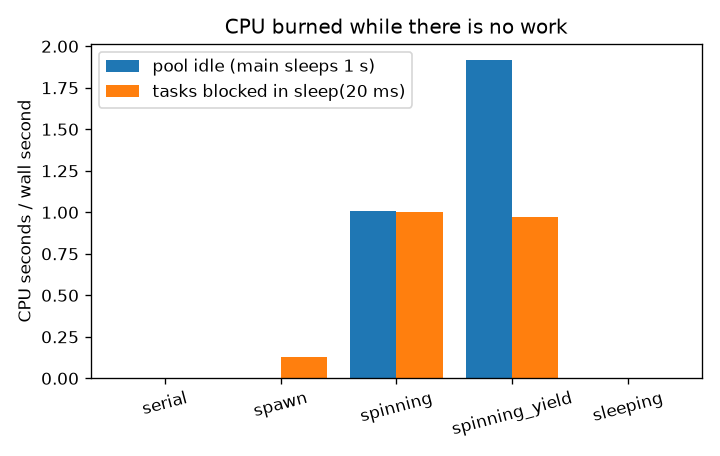
\includegraphics[width=\linewidth]{cpu_burn.png}\caption{CPU 浪费}\end{subfigure}
\begin{subfigure}{0.49\linewidth}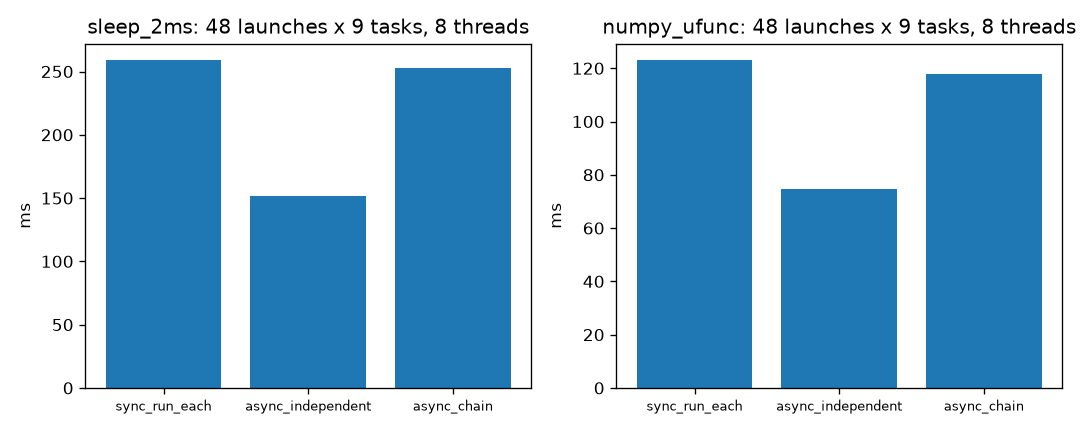
\includegraphics[width=\linewidth]{async_overlap.png}\caption{异步重叠}\end{subfigure}
\caption{Python \texttt{threading} 版（本机 8 逻辑处理器）的四张图，数据见 \texttt{artifacts/raw/*.csv}。}
\label{fig:python}
\end{figure}

Python 版在本机测得：睡眠池 8 个空任务每次 launch 38.7~µs，spawn 3169~µs，纯自旋池 31--50~ms；空闲时纯自旋只烧 1.006 个核；
48 个 9 任务的 launch 用 async 从 259~ms 降到 152~ms。与 C++ 版对照（\cref{fig:python}）：
\begin{itemize}
\item 自旋池：在 Python 中最慢（自旋线程要等 5~ms 的 GIL 切换间隔才让出解释器），在 C++ 中唤醒最快（0.783~µs）。
\item 空闲 CPU：Python 纯自旋只烧 1 个核（GIL 把自旋也串行化了），C++ 烧满 12 个核。
\item 异步尾部填充：两者都得到接近 \cref{eq:tail} 的收益（Python 1.71 倍，理想 1.78；C++ 1.64 倍，理想 1.83），因为这是调度层面的效应，与执行引擎无关。
\item false sharing：Python 对象不在可控的 cache line 上，无法测量；C++ 测得 19 倍。
\end{itemize}
所以，Python 版可以用来验证调度算法的正确性和尾部效应，但回答不了任何与``等待策略''或``硬件''有关的问题。

%====================================================================
\section{面试专题}
\label{sec:interview}

\subsection{20 秒版本}

任务系统有三笔开销。第一笔是让线程开始干活：spawn 约 16~µs/线程，睡眠池约 10~µs，自旋池不到 1~µs。
第二笔是每个任务的分发：分发计数器是一个被所有核争抢的 cache line，约 15~ns 起步，CAS 冲突时可到 500~ns。第三笔是等待时的 CPU：自旋会烧满所有核。
我在 12 核上实测，常驻池把 launch 从 200~µs 降到 1--13~µs；自旋只有在线程数小于空闲核数时才划算，留一个核给调用者能让它快 1.7 倍，超额订阅再加上锁会慢 766 倍；
async 依赖图让独立 launch 互相填尾，13 任务/12 线程时快 1.64 倍，树形归约达到 work 下界的 96\%。

\subsection{追问与答案}

\begin{iqbox}{自旋池和睡眠池哪个快？}
\textbf{答}：要看等待时间有多长、核是否独占。唤醒延迟上自旋快一个数量级（单任务 launch 0.783 对 10.8~µs），所以每次 launch 只有几微秒工作的测试（\texttt{super\_\allowbreak{}super\_\allowbreak{}light}）只有自旋池能赢串行。
但自旋空闲时会烧满所有核，线程数一旦超过空闲核数，自旋线程就会抢走干活线程的 CPU。生产系统用的是``先自旋一段（约等于一次上下文切换的代价），再睡眠''的混合策略。\\
\textbf{常见错答}：``自旋永远更快''，或者``自旋浪费 CPU，所以永远不该用''。本文两个方向的反例都有：64 个空任务时自旋池（34.0~µs）反而比睡眠池（12.7~µs）慢，原因是 CAS 争用，而不是等待方式。
\end{iqbox}

\begin{iqbox}{为什么每次 \texttt{run} 都建线程不行？代价有多大？}
\textbf{答}：建线程要 \texttt{clone}、分配栈、等内核调度，结束时还要 \texttt{join}。实测 1 个线程 28.6~µs、12 个线程 204~µs，约 16~µs/线程。
对 \texttt{math\_\allowbreak{}operations\_\allowbreak{}in\_\allowbreak{}tight\_\allowbreak{}for\_\allowbreak{}loop}（2000 次 launch，每次不到 2~µs 有用工作）来说，这意味着 387~ms 对串行的 5.14~ms。
但在计算量大的 launch（mandelbrot，每次约 80~ms）里，这笔开销可以忽略，spawn 甚至最快。\\
\textbf{常见错答}：``线程创建要毫秒级''（那是 Python，C++ 是十几微秒）；或者``spawn 版应该静态划分任务''，而静态划分在 \texttt{ping\_\allowbreak{}pong\_\allowbreak{}unequal} 这种不均衡负载上会更差。
\end{iqbox}

\begin{iqbox}{线程池里怎样防止 worker 把上一个 launch 的计数器用到下一个 launch 上？}
\textbf{答}：这是常驻池最容易写错的竞态。我把 generation 与下一个任务下标打包进一个 64 位原子变量，用 CAS 认领，generation 一变 CAS 就失败。
调用者只有在 \texttt{done == total} 后才发布下一个 generation，所以认领成功后读到的 runnable 一定属于同一个 launch。另一种做法是每个 launch 分配独立的状态对象，用引用计数回收。\\
\textbf{常见错答}：``先把 \texttt{next} 清零再改 runnable''。不同变量的写入顺序，挡不住一个已经读了旧状态、尚未执行 \texttt{fetch\_\allowbreak{}add} 的 worker。
\end{iqbox}

\begin{iqbox}{条件变量为什么要在 \texttt{while}（或带谓词的 \texttt{wait}）里等？什么是 lost wakeup？}
\textbf{答}：因为 \texttt{wait} 可能虚假唤醒，被唤醒时条件也可能已经被别的线程消费了，所以必须重新检查谓词。
lost wakeup 是指在``检查条件''和``开始睡眠''之间，别人恰好发了通知：如果修改条件时不持有同一把锁，通知就可能落空，线程永远睡下去。
本文所有共享谓词（generation、\texttt{finished\_\allowbreak{}gen}、ready 队列）都在锁内修改。\\
\textbf{常见错答}：``用 \texttt{notify\_\allowbreak{}all} 就不会丢''。丢不丢与 \texttt{notify\_\allowbreak{}one}/\texttt{all} 无关，而与是否在锁内修改条件有关。
\end{iqbox}

\begin{iqbox}{\texttt{runAsyncWithDeps} 为什么能快？快多少有上限吗？}
\textbf{答}：收益有两种。一是填尾：$K$ 个 $n$ 任务的 launch，同步需要 $K\lceil n/P\rceil$ 轮，async 只要 $\lceil Kn/P\rceil$ 轮，13 任务/12 线程时理想 1.83 倍、实测 1.64 倍。
二是让 DAG 中不相关的分支并行：树形归约 14.8~ms，接近 work 下界 $T_1/P = 14.25$~ms，而同步版被逐层屏障卡在 27.1~ms。上限由 Brent 定理给出：$T_P \ge \max(T_1/P, T_\infty)$。\\
\textbf{常见错答}：``async 让单个任务变快''，其实任务本身一点没快，省掉的是空闲；或者认为链式依赖也能加速（实测 26.9 对 27.1~ms，没有变化）。
\end{iqbox}

\begin{iqbox}{什么是 false sharing？你怎么测出来的？}
\textbf{答}：不同线程写同一个 64~B cache line 上的不同变量，一致性协议就会把整行在核之间来回迁移。我实测 12 个线程各自 \texttt{fetch\_\allowbreak{}add} 自己的计数器，
放在同一行时 113~ns/次，各占一行（\texttt{alignas(64)}）时 5.89~ns，差 19 倍。测量时两种布局必须跑同一份代码、只改步长：我的第一版用了不同的数据结构，单线程就差 6.7 倍，完全掩盖了效应。\\
\textbf{常见错答}：``false sharing 是两个线程写同一个变量''（那是 true sharing）；``加 \texttt{volatile} 就能解决''；或者以为 SMT 兄弟之间也有 false sharing，其实它们共享 L1，原子版本实测没有差别（12.6 对 13.0~ns）。
\end{iqbox}

\begin{iqbox}{动态分配任务用互斥锁、原子计数器还是分块？}
\textbf{答}：任务小的时候用分块。12 线程、空任务时，互斥锁 93.5~ns/项，原子 \texttt{fetch\_\allowbreak{}add} 15.0~ns，每次取 64 个 0.683~ns。单个原子计数器是全局串行点，吞吐停在一次 cache line 迁移的约 15~ns；
每项 30~ns 工作时，原子版完全不扩展（45.5~ns/项），分块后与静态划分相同（4.26 对 4.66~ns）。所以任务要么足够大（远大于 15~ns × 线程数），要么按块取，要么改成每线程本地队列加 work stealing。\\
\textbf{常见错答}：``原子操作是无锁的，所以可以无限扩展''。无锁不等于无争用，CAS 循环比 \texttt{fetch\_\allowbreak{}add} 还差，因为失败要重试（自旋池每个空任务 494~ns）。
\end{iqbox}

\begin{iqbox}{线程数应该等于核数吗？}
\textbf{答}：对睡眠池，等于核数甚至加上 SMT 兄弟都可以（24 个 worker 让 mandelbrot 快 1.73 倍）。对自旋池，应该是核数减 1，或者让调用者也干活：
12 个 worker 加上自旋的调用者，就是 13 个忙线程挤 12 个核，被换下的 worker 手里的任务要等一个时间片，粒度实验中出现了 32.0~ms 的平台，换成 11 个 worker 后降到 18.7~ms。
超额订阅时，带锁的自旋调度器会慢 766 倍（锁持有者被抢占）。\\
\textbf{常见错答}：``越多越好，反正操作系统会调度''。对自旋线程，操作系统并不知道它在空转。
\end{iqbox}

\begin{iqbox}{如果任务粒度极不均匀、还会动态产生新任务，你的设计怎么改？}
\textbf{答}：换成每线程一个双端队列的 work stealing（Cilk、TBB、Go runtime）。本线程从队尾 push/pop，没有争用，cache 局部性也好；空闲线程从别人的队首偷任务。
Blumofe--Leiserson 证明了它的期望时间为 $T_1/P + O(T_\infty)$，偷取次数为 $O(P\,T_\infty)$。本文的全局 ready 队列在 12 线程上够用，但粒度实验显示 262144 个任务时全局锁让 async 版慢到 129~ms，这正是 work stealing 要解决的问题。\\
\textbf{常见错答}：``给全局队列换一个更快的锁''。问题出在全局串行点本身，而不是锁的实现。
\end{iqbox}

\subsection{STAR 故事}

\textbf{情境}：CS149 Assignment 2 要求实现任务系统，并比较自旋、睡眠和依赖图调度；仓库原有 Python 版的结论被 GIL 主导，而服务器是 7 个代理共享的 16-CPU 容器。
\textbf{任务}：用 C++ 实现官方 API 下的 6 个系统与 20 个测试，在 60 分钟的服务器窗口内拿到可重复、可追溯的数据，回答官方问题并补充 9 组实验。
\textbf{行动}：用 generation 与下标打包的 CAS 解决 launch 之间的竞态，所有测试都带结果校验与超时；先在本机跑通 120 个组合确认正确，再在 12 个独占核上跑 3 轮。
看到自旋池在 12 线程时反而比睡眠池慢一倍、粒度曲线停在整齐的 32.0~ms 后，我推断是调用者线程在和 worker 分时，于是追加了 11 个 worker 的对照实验来验证。
发现第一版 false sharing 微基准单线程就差 6.7 倍后，改成同一份代码只改步长，重新测量。
\textbf{结果}：launch 开销从 204~µs（spawn）降到 0.783--12.7~µs；定位了 32.0 → 18.7~ms 的``调用者占核''问题和 766 倍的锁持有者抢占问题；
async 依赖图让树形归约达到 work 下界的 96\%；false sharing 测得 19 倍。所有数字都可以从 \texttt{artifacts/raw/cpp/} 的 jsonl 复算。

%====================================================================
\section{局限}
\label{sec:caveat}

\begin{caveatbox}
\begin{itemize}
\item 服务器是共享宿主机：16 个 CPU 的 cgroup 配额由 7 个代理共享，其他代理的不绑核进程可能落在本文的 12 个核上，配额用满时整个容器会被暂停（第 1 轮中有 10 个周期被 throttle）。
自旋类实现每个核都在跑，最容易被这两种干扰放大；文中自旋池在 12 线程下的若干``反常''数字至少部分来自这里，
不能推广成``自旋池在独占机器上也比睡眠池慢''。
\item 不能从\cref{fig:scaling} 推出``睡眠池在 mandelbrot 上不扩展''：2--8 线程时睡眠池、spawn 与 async 睡眠池都只有 1.5--2.9 倍，而自旋池有 1.9--6.3 倍，3 轮都复现。
\cref{fig:anomaly} 的分析排除了唤醒开销、负载不均和实现缺陷（本机对照中四种常驻池差不到 5\%），定位到``worker 的每条指令更贵''；
剩下的频率管理与 SMT 兄弟被占两个候选，没有 \texttt{turbostat} 无法区分。
\item 官方 \texttt{tests.h} 不在手边，测试是按结构重写的，规模经过缩放（例如 fib(23)）。各系统之间的相对关系可比，绝对时间不能与官方参考解比较。
\item 调用者线程不绑核；本文用 11 个 worker 的对照实验量化了调用者占核的影响（单轮），没有实现``调用者也参与执行任务''的设计。
\item \texttt{BulkLaunchState} 的 \texttt{state\_\allowbreak{}}、\texttt{total\_\allowbreak{}}、\texttt{done\_\allowbreak{}} 相邻存放，很可能处于同一个 cache line，调用者自旋读 \texttt{done\_\allowbreak{}} 时会和 worker 的 CAS 抢这一行；
本文没有做拆分 cache line 的消融实验，空任务开销中有多少来自这里没有量化。
\item \texttt{volatile} 版 false sharing 只差 1.2--1.4 倍、SMT 兄弟上差 3.4 倍，文中给出的 store buffer 和 memory ordering 解释是推测，没有用性能计数器验证。
\item 没有实现 work stealing；Part~B 用一把全局锁，任务极小且线程多时锁会成为瓶颈。
\item 单线程 turbo 频率高于全核频率，本文没有锁频，所以多线程加速比天然低于线性。
\end{itemize}
\end{caveatbox}

%====================================================================
\section{结论}

本文用 C++17 实现了 CS149 Assignment 2 要求的全部任务系统和依赖图调度器，并在 12 个独占物理核上回答了作业的核心问题。
一次 bulk launch 的成本由三部分组成：让线程开始干活、每个任务的分发，以及等待时花掉的 CPU。读者最该带走的是下面几点。

常驻线程池消除了第一部分的大头（200~µs → 1--13~µs）。自旋用 CPU 换延迟，只有在线程数不超过空闲核数时才划算；留一个核给调用者、不在自旋路径上持锁，是两条最实用的规则。
分发计数器是一个被所有核争抢的 cache line，所以任务粒度必须远大于一次行迁移（约 15~ns）乘以线程数，否则就要按块分发。
依赖图调度把同步执行的逐层屏障换成了真正的 DAG，独立 launch 互相填尾，树形归约达到 work 下界的 96\%。

这些结论与 Brent 的 work/span 界、缓存一致性的串行化模型以及 work stealing 的理论都对得上，
也解释了为什么 TBB、Cilk 等生产级运行时都采用``调用者参与执行、每线程一个队列、先自旋后睡眠''的组合。

\begin{thebibliography}{99}
\bibitem{cs149} K. Fatahalian, K. Olukotun. CS149: Parallel Computing, Stanford University, Fall 2024. Assignment 2: Scheduling Task Graphs on a Multi-Core CPU. \url{https://github.com/stanford-cs149/asst2}.
\bibitem{blumofe} R. D. Blumofe, C. E. Leiserson. Scheduling Multithreaded Computations by Work Stealing. \emph{Journal of the ACM}, 46(5):720--748, 1999.
\bibitem{cilk5} M. Frigo, C. E. Leiserson, K. H. Randall. The Implementation of the Cilk-5 Multithreaded Language. In \emph{PLDI}, 1998.
\bibitem{tbb} J. Reinders. \emph{Intel Threading Building Blocks: Outfitting C++ for Multi-core Processor Parallelism}. O'Reilly, 2007.
\bibitem{mcs} J. M. Mellor-Crummey, M. L. Scott. Algorithms for Scalable Synchronization on Shared-Memory Multiprocessors. \emph{ACM Transactions on Computer Systems}, 9(1):21--65, 1991.
\bibitem{herlihy} M. Herlihy, N. Shavit. \emph{The Art of Multiprocessor Programming}. Morgan Kaufmann, 2008.
\bibitem{drepper} U. Drepper. What Every Programmer Should Know About Memory. Red Hat, 2007.
\bibitem{amdahl} G. M. Amdahl. Validity of the Single Processor Approach to Achieving Large Scale Computing Capabilities. In \emph{AFIPS Spring Joint Computer Conference}, 1967.
\bibitem{brent} R. P. Brent. The Parallel Evaluation of General Arithmetic Expressions. \emph{Journal of the ACM}, 21(2):201--206, 1974.
\bibitem{graham} R. L. Graham. Bounds on Multiprocessing Timing Anomalies. \emph{SIAM Journal on Applied Mathematics}, 17(2):416--429, 1969.
\bibitem{anderson} T. E. Anderson. The Performance of Spin Lock Alternatives for Shared-Memory Multiprocessors. \emph{IEEE Transactions on Parallel and Distributed Systems}, 1(1):6--16, 1990.
\bibitem{ousterhout} J. K. Ousterhout. Scheduling Techniques for Concurrent Systems. In \emph{ICDCS}, 1982.
\bibitem{chaselev} D. Chase, Y. Lev. Dynamic Circular Work-Stealing Deque. In \emph{SPAA}, 2005.
\bibitem{torrellas} J. Torrellas, M. S. Lam, J. L. Hennessy. False Sharing and Spatial Locality in Multiprocessor Caches. \emph{IEEE Transactions on Computers}, 43(6):651--663, 1994.
\bibitem{tullsen} D. M. Tullsen, S. J. Eggers, H. M. Levy. Simultaneous Multithreading: Maximizing On-Chip Parallelism. In \emph{ISCA}, 1995.
\bibitem{intel} Intel. Intel 64 and IA-32 Architectures Optimization Reference Manual, 2023.
\end{thebibliography}


\end{document}
